%-------------------------------------------
% Packages Used
%-------------------------------------------
\documentclass[12pt, a4paper]{article}

% === Basic Document and Encoding ===
\usepackage[T1]{fontenc}        % Font encoding
\usepackage{geometry}           % Page size and margins
\usepackage{setspace}           % Line spacing
\usepackage{lipsum}             % Dummy text

% === Math and Symbols ===
\usepackage{amsmath}            % Math environments
\usepackage{amsfonts}           % Math fonts
\usepackage{mathrsfs}           % Script fonts
\usepackage{eqnarray}           % Eqnarray environment

% === Tables and Tabulars ===
\usepackage{booktabs}           % Professional tables
\usepackage{threeparttable}     % Table footnotes
\usepackage{longtable}          % Long tables
\usepackage{multirow}           % Multirow cells
\usepackage{diagbox}            % Diagonal boxes in tables
\usepackage{tabularray}         % Tabularray tables
\usepackage[table]{xcolor}      % Table cell coloring

% === Figures and Graphics ===
\usepackage{graphicx}           % Images
\usepackage{float}              % Customizing float positions
\usepackage{subcaption}         % Subfigures
\usepackage{caption}            % Caption customization
\usepackage{afterpage}          % Place floats after page break
\usepackage{adjustbox}          % Adjustable boxes for tables and figures

% === Algorithms and Code ===
\usepackage{algorithm}          % Algorithm floats
\usepackage{algorithmicx}       % Algorithmicx package
\usepackage{algpseudocode}      % Pseudocode
\usepackage{listings}           % Code listings

% === Document Structure and Sections ===
\usepackage{titlesec}           % Section formatting
\usepackage[title]{appendix}    % Appendix environment
\usepackage{authblk}            % Author affiliations
\usepackage{chngcntr}           % Change counters

% === Text Formatting and Lists ===
\usepackage{enumitem}           % Custom lists
\usepackage[]{ragged2e}         % Ragged right text
\usepackage{comment}            % Large comment blocks

% === Landscape and Page Layout ===
\usepackage{lscape}             % Landscape tables
\usepackage{pdflscape}          % Landscape pages

% === Bibliography and Citations ===
\usepackage[backend=biber, citestyle=apa, bibstyle=apa, maxbibnames=20, date=year, urldate=year, alldates=year]{biblatex} % Bibliography management
\usepackage{csquotes}           % Context-sensitive quotation

% === Hyperlinks and Colors ===
\usepackage[colorlinks=true, allcolors=blue]{hyperref} % Hyperlinks

% === Miscellaneous ===
\usepackage{orcidlink}          % ORCID iDs
\usepackage{lineno}             % Line numbers
\usepackage[none]{hyphenat}     % Disable hyphenation
\usepackage{csvsimple}          % Import CSV to LaTeX

%-------------------------------------------
% Document Preamble
%-------------------------------------------

% === Bibliography Reference ===
\addbibresource{refs.bib} % Reference .bib file
%\bibliographystyle{apa}

% === Page Layout and Spacing ===
\geometry{a4paper,
        top=1in,
        bottom=1in,
        left=1in,
        right=1in,
        marginparwidth=0.5in
        }

\onehalfspacing % 1.5 line spacing
\setlength{\parskip}{0.5\baselineskip} % Vertical space between paragraphs
\setlength{\parindent}{1.5em} % Paragraph indentation

% === Section Formatting ===
\titleformat{\section} % Redefine section numbering format
{\normalfont\Large\bfseries}{\thesection.}{1em}{}

% === Line Numbering ===
% \renewcommand\linenumberfont{\normalfont\scriptsize\sffamily\color{blue}}
% \linenumbers % Enable line numbering
% \rightlinenumbers % Right-align; comment this line for left alignment.

% === Custom Commands and Environments ===
% Define a new command for the fourth-level title.
\newcommand{\subsubsubsection}[1]{%
  \vspace{\baselineskip} % Add some space
  \noindent\textbf{#1\\}\quad % Adjust formatting as needed
}

% Change the position of the table caption above the table
\captionsetup[table]{position=top} % caption position for tables

% Make Table and Figure labels bold and change separator from colon to period
\captionsetup{labelfont=bf, labelsep=period} % Make all caption labels (Table X, Figure X) bold and use period separator

% Define the unnumbered list
\makeatletter
\newenvironment{unlist}{%
  \begin{list}{}{
    \setlength{\labelwidth}{0pt}%
    \setlength{\labelsep}{0pt}%
    \setlength{\leftmargin}{2em}%
    \setlength{\itemindent}{-2em}%
    \setlength{\topsep}{\medskipamount}%
    \setlength{\itemsep}{3pt}%
  }%
}{%
  \end{list}%
}
\makeatother


% === Miscellaneous Settings ===
% Suppress the warning about \@parboxrestore
%\pdfsuppresswarningpagegroup=1

% Suppress the warning about overfull boxes
\sloppy

%-------------------------------------------
% Title and Abstract
%-------------------------------------------
\title{\textbf{Are Older Adults in China Living Longer Happy Years? A Cohort-Based Multistate Analysis, 2002–2018}}
\author[*]{\small Yunxiang Wan\orcidlink{0009-0003-7482-7991}}
\author[1]{\small Marilia Nepomuceno}
\author[2]{\small Marwan Al Qays Bousmah}

\affil[1]{\small{Max Planck Institute for Demographic Research, Rostock, Germany, 18057}}
\affil[2]{\small{French Institute for Demographic Studies, Paris, France, 93300}}
%\affil[3]{\small{Max Planck Institute for Demographic Research, Rostock, Germany, 18057}}
\affil[*]{Corresponding author: \href{mailto:wan@demogr.mpg.de}{wan@demogr.mpg.de}}
\date{}

\begin{document}
\newpage

% === Title ===
\maketitle

% === Abstract ===
\begin{abstract}
  \noindent\textbf{Objective:} As China's population ages and life expectancy rises, a critical question is whether older adults are living longer happy years. This study examines changes in happy life expectancy (HapLE) across birth cohorts and investigates socioeconomic disparities in these changes.

  \noindent\textbf{Methods:} Using data from the Chinese Longitudinal Healthy Longevity Survey (CLHLS) for 2002–2018, we applied multistate life table models to estimate partial-cohort HapLE (PC-HapLE) for four age ranges. We compared earlier cohorts with later cohorts born 10 years apart and stratified analyses by gender, education, and urban-rural residence.

  \noindent\textbf{Results:} Results show that later cohorts experienced a significant increase in the number and proportion of happy years, driven by a "compression of unhappiness." However, these gains were unequally distributed. Urban older adults saw substantial and significant increases in PC-HapLE across all age groups, whereas gains for rural residents were modest and often statistically insignificant. Similar patterns of widening inequality were found by education and gender, with literate individuals and women experiencing greater improvements.

  \noindent\textbf{Conclusion:} While Chinese older adults are living longer happy years on average, this positive trend masks widening inequalities. Socioeconomic development has disproportionately benefited urban, educated, and female older adults, creating a growing "happiness gap." Policies must shift from merely extending lifespan to promoting equitable aging by addressing these disparities.
  \vspace{1em}

  \noindent\textbf{Keywords}: happy life expectancy, multi-state model, cohort analysis, China
\end{abstract}


%-------------------------------------------
% Highlights
%-------------------------------------------
% \newpage
% \section*{Highlights}
% \begin{itemize}
%     \item Problem and solution
%     \item Method
%     \item Result 1 / Recommendations / Policy Implications
%     \item Result 2 / Recommendations / Policy Implications
%     \item Result 3 / Recommendations / Policy Implications / Conclusion
% \end{itemize}

%-------------------------------------------
% Introduction
%-------------------------------------------
\newpage
\section{Introduction}
China has undergone a rapid process of population aging. In 2023, the number of individuals aged 65 and older reached 210 million, constituting over 15\% of the total population—a proportion that has doubled in just over two decades \autocite{nationalbureauofstatisticsofchina.2023.china}. Projections estimate this figure will climb to 390 million by 2050, comprising nearly 30\% of the nation's population \autocite{unitednations.2024.world}. This demographic shift has been accompanied by triumphs in life expectancy (LE), which increased from 43.8 years in 1950 to 78.0 years in 2023 \autocite{unitednations.2024.world}. However, these gains in longevity raise a critical, yet less understood question: are these added years of life also happy years? Answering this is crucial for shaping effective aging policies that move beyond merely extending longevity to enhancing the quality of those added years.

To address this question, this study presents a novel, cohort-based examination of trends in happy life expectancy (HapLE) among older adults in China. This approach directly extends the only two foundational, yet limited studies on HapLE in China. The first, by Duan and Chen \autocite{duan.2020.happy}, pioneered the use of HapLE in China and, using a period-based analysis, found an overall "compression of unhappiness"—a pattern where the proportion of life spent in an unhappy state decreases over time. The second, by Wan and Jiang \autocite{wan.2024.socioeconomic}, documented significant static socioeconomic inequalities in HapLE at a specific period of time. Our study builds upon and advances this work in two fundamental ways. First, by shifting the analysis from a period to a cohort perspective, we aim to better capture the lived experiences of successive generations \autocite{payne.2022.expansion}. Second, by moving from a static to a dynamic analysis of inequality, we examine how these socioeconomic gaps evolve across birth cohorts.

We explore these questions by using multistate life table models on nationally representative longitudinal data from the Chinese Longitudinal Healthy Longevity Survey (CLHLS) from 2002 to 2018. Our findings reveal an optimistic aggregate trend: Chinese older adults are, on average, living longer happy years, a gain primarily driven by a significant "compression of unhappiness." However, this positive narrative masks a more troubling counter-trend of widening disparities. The improvements in happiness have disproportionately benefited urban, educated, and female older adults, creating a growing "happiness gap" that challenges the notion of equitable aging.

The rest of this paper is structured as follows. We first review the relevant literature and identify key research gaps. We then describe our data and analytical methods, followed by a presentation of the results. We conclude by discussing our findings and the strengths and limitations of our study.

%-------------------------------------------
% Literature Review
%-------------------------------------------
\section{Literature Review}

\subsection{Past Research}
The study of population aging has long been driven by two critical concerns: the length of life and the quality of health during those years. To address these concerns, healthy life expectancy (HLE) emerged as a vital and widely adopted measure, shedding light on the true quality of life in societies with aging populations \autocite{sanders.1964.measuring}. The central debate has revolved around whether gains in life expectancy are accompanied by a "compression of morbidity"—a shorter period of ill-health before death—or an "expansion of morbidity," where longer lives are spent in poorer health \autocite{fries.1980.aging,gruenberg.1977.failures}. Consequently, HLE and its variants, such as disability-free life expectancy (DFLE) and morbidity-free life expectancy (MFLE), have become standard indicators for evaluating population quality of life and well-being.

However, while physical health is a fundamental component of well-being, it does not encompass the full spectrum of an individual's life experience \autocite{yang.2008.long}. The World Health Organization defines quality of life as a multidimensional concept that includes not only physical health but also psychological state, social relationships, and personal beliefs \autocite{thewhoqolgroup.1998.development}. Recognizing this, a growing body of scholars argues that a singular focus on health and disability overlooks the crucial cognitive and emotional dimensions of aging \autocite{george.2010.still}. Happiness is a cognitive, global judgment of the quality of life, which is defined as the extent to which an individual positively evaluates their overall life as a whole \autocite{veenhoven.1996.study}. Analogous to HLE, happy life expectancy (HapLE) has emerged as a powerful summary measure that integrates longevity with happiness \autocite{yang.2008.long}. HapLE decomposes total life expectancy into years lived in happy versus unhappy states, offering a more comprehensive answer to the critical question of whether gains in life quantity are also gains in life quality. By examining HapLE, we can move beyond the narrow focus on disease and disability to assess whether societies are fostering environments where older adults not only survive but also thrive \autocite{yang.2008.long,wan.2024.socioeconomic}.

Since its introduction, research on HapLE trends has shown a complex picture worldwide. Early research from the United States painted an optimistic narrative of progress, finding that between 1970 and 2000, Americans were living both more years and a larger proportion of their lives happily \autocite{yang.2008.long,yang.2010.increment}. This "compression of unhappiness" was also documented in the Netherlands \autocite{perenboom.2004.trends}. However, this narrative of progress has been challenged. Research in West Germany revealed a paradox: while absolute happy years increased, the proportion of life spent satisfied actually declined due to a deterioration in end-of-life well-being \autocite{nemitz.2022.increasing}. Moreover, HapLE trends in post-communist nations like Russia have been highly volatile, fluctuating with socioeconomic turmoil \autocite{minagawa.2022.trends}. These diverging international findings underscore that HapLE trends are not monolithic but are deeply embedded in national contexts.

\subsection{Chinese Context}

In the unique context of China's rapid socioeconomic transformation, the trajectory of population well-being has been a subject of intense scholarly debate. One influential line of inquiry, rooted in the “Easterlin paradox,” has argued that the country's unprecedented economic growth, particularly from the 1990s to the early 2000s, did not translate into a corresponding rise in life satisfaction\autocite{easterlin.2012.chinas,graham.2017.happiness,knight.2011.does}. This disconnect has been attributed to the social disruptions accompanying market reforms, such as rising unemployment, growing income inequality, and the dissolution of the “iron rice bowl” social safety net \autocite{easterlin.2012.chinas,li.2014.time}. However, more recent evidence suggests a reversal of this trend. Several studies document a significant upswing in happiness levels since the early 2000s \autocite{cai.2023.does,wang.2023.hierarchical}, a recovery often linked to the maturing of China's social security systems and a narrowing of the urban-rural development gap \autocite{payne.2022.expansion}. Within this broader debate, the lone study on HapLE trends in China, a period-based analysis by Duan and Chen \autocite{duan.2020.happy}, offers a critical insight, finding evidence of an overall "compression of unhappiness" for the general adult population.

However, this aggregate picture of improving well-being, whether viewed through happiness trends or HapLE, may conceal deep and persistent inequalities. Socioeconomic status acts as a fundamental determinant of life chances, shaping access to the resources required for a happy and healthy life, particularly in old age. The most prominent fault line in Chinese society is the urban-rural divide. This institutionalized disparity, originating from the hukou system, has long produced significant gaps in income, healthcare, and educational opportunities \autocite{guo.2024.regional,liu.2019.are}. While research has noted a "rural-urban paradox" where rural elderly sometimes report better health-related outcomes \autocite{jiao.2019.inequality,zhang.2022.trends}, the structural disadvantages faced by rural populations in terms of economic and social resources are well-documented \autocite{wang.2020.gap} and are expected to extend to happiness.

Beyond a person's place of residence, education serves as another key stratifying mechanism. As a primary indicator of socioeconomic status, education equips individuals with the capacity to navigate complex healthcare and social welfare systems, access more stable and higher-paying employment, and build stronger social networks, all of which are crucial determinants of well-being \autocite{payne.2022.expansion}. Studies using Chinese data have consistently identified education as a significant predictor of subjective well-being among older adults \autocite{cheng.2021.sociodemographic}. A recent analysis of HapLE in China confirmed that significant educational inequalities exist, with more educated older adults living longer happy lives \autocite{wan.2024.socioeconomic}. While these period-based studies and static analyses have been foundational in identifying the existence of a "happiness gap," they leave a critical question unanswered: how have these inequalities evolved across generations? It remains unknown whether the benefits of China’s recent socioeconomic progress have been distributed equitably, leading to a narrowing of these disparities for later-born cohorts, or if advantaged groups have disproportionately gained, leading to a widening gap.

\subsection{Current Study}
The preceding review reveals two critical gaps in the understanding of quality of life among China's aging population. First, while existing research has debated aggregate HapLE trends, its reliance on period-based analyses offers an incomplete picture \autocite{duan.2020.happy}. Period-based estimates are valuable for monitoring population-level shifts but cannot fully capture the lived experiences of individuals as they age, as these estimates based on data from a combination of different cohorts. A cohort perspective, by contrast, tracks the experiences of specific generations, providing clearer insights into whether later-born groups are living better than their predecessors \autocite{payne.2022.expansion}.

Second, while studies have established the existence of significant, static socioeconomic disparities in happiness and HapLE at single period of time \autocite{wan.2024.socioeconomic}, they do not address the dynamics of this inequality. It remains an open question whether the "happiness gap" between advantaged and disadvantaged groups has narrowed or widened across successive birth cohorts. Answering this requires a dynamic analysis that examines whether the benefits of China’s socioeconomic development—such as expanded social security and improved healthcare—have been equitably distributed or if they have disproportionately favored those with more resources \autocite{liu.2019.are}.

To address these limitations, this study makes two primary contributions. First, by employing a cohort-based multistate life table approach, we move beyond period comparisons to assess whether later-born cohorts of Chinese older adults are living longer happy years. Second, we conduct a dynamic analysis of inequality, examining how trends in HapLE differ by urban-rural residence, education level, and gender across cohorts. By doing so, we aim to provide robust evidence on both the overall progress and the equity of quality-of-life changes during China’s rapid aging process.

%-------------------------------------------
% Method
%-------------------------------------------

% === Data ===
\section{Method}
\subsection{Data}
This study used data from CLHLS \autocite{centerforhealthyaginganddevelopmentstudies.2020.chinese}. CLHLS covers 23 provinces, municipalities, and autonomous regions across China and is the first and longest-running social science survey of its kind in the country. The survey includes approximately 85\% of the elderly population in China, ensuring strong representativeness \autocite{gu.2008.general,zeng.2008.introduction}. CLHLS was launched with a baseline survey in 1998 and has since conducted longitudinal follow-ups in 2000, 2002, 2005, 2008/2009, 2011/2012, 2014, and 2017/2018, accumulating eight waves of longitudinal data spanning two decades. In the 1998 and 2000 waves, the survey targeted individuals aged 80 and above, while from 2002 onward, the age range was expanded to include those aged 65 and older. The analyses in this study used individuals who participated in at least two of the three waves conducted in 2002, 2005, and 2008, or who passed away between these waves (N=6371) and individuals who participated in at least two of the three waves conducted in 2011/2012 (2012 thereafter), 2014, and 2017/2018 (2018 thereafter), or who passed away between these waves (N=4221).

% === Measures ===
\subsection{Measures}
This study used HapLE as the outcome to examine cohort trends in longevity and happiness among older adults in China. By decomposing LE into the number of years lived in happy and unhappy states, both HapLE and unhappy life expectancy (UHapLE) can be derived. HapLE can be viewed from an absolute perspective, referring to the number of years an individual is expected to live in a happy state, or from a relative perspective, as the proportion of HapLE in LE (HapLE\%).

Happiness was assessed using a single-item measure of life satisfaction in CLHLS. The terms subjective well-being, life satisfaction, and happiness are often considered interchangeable in relevant literature \autocite{easterlin.2021.growth,yang.2008.long}. This measurement approach has been widely applied in large-scale surveys due to its simplicity and effectiveness and has demonstrated high reliability and validity in assessing individual well-being \autocite{baur.1983.stability,lucas.2018.shortterm}. Specifically, CLHLS evaluated respondents' life satisfaction through the question: "How do you feel about your life at present?" Responses were rated on a five-point scale, where 1 represents "very good" and 5 represents "very bad." For analytical convenience and consistency with existing research \autocite{duan.2020.happy,wan.2024.socioeconomic}, this study dichotomized the variable: respondents answering 1 or 2 were classified as "happy," while those answering between 3 and 5 were categorized as "unhappy." CLHLS primarily collected mortality information from official death certificates when available. If an official certificate was not accessible, mortality data were obtained from local community committees or reports from close relatives. When a respondent's death was confirmed in a specific survey wave, their survival status in that wave was recorded as "dead."

This study included four covariates: age, sex, urban-rural residence, and education level. Urban-rural residence is closely linked to inequalities in healthcare access, income levels, economic growth, and infrastructure development in Chinese society, which have been extensively studied \autocite{liu.2019.are}. Education level is a well-established indicator of socioeconomic status and serves as a key predictor of an individual's social and economic conditions \autocite{wan.2024.socioeconomic}. In this study, urban-rural residence and educational level were further used in subgroup analyses. Regarding variable definitions, age was treated as a continuous variable, and sex was categorized as men or women. Urban-rural residence was measured at baseline using the survey question: "Where do you currently live?" Response options included "city," "town," and "rural area." In this analysis, the "city" and "town" categories were combined into "urban." Educational level was coded based on respondents' years of schooling at baseline, derived from the survey question: "How many years of formal education have you completed in total?" Respondents with zero years of schooling were classified as "illiterate," while those with more than zero years were categorized as "literate."

% === Model ===
\subsection{Model}
This study used a method for estimating state-specific partial-cohort life expectancy (PC-LE), which is calculating total life expectancy within a specified age range for a given cohort, as well as the expected years lived in the happy state. This method had been used to examine trends in healthy life expectancy (HLE), disability-free life expectancy (DFLE), and morbidity-free life expectancy (MFLE) across successive birth cohorts \autocite{liu.2019.are,payne.2022.expansion,payne.2019.expansion,shen.2023.disability}. Compared to estimates of full-cohort life expectancy, PC-LE estimates do not require data from fully extinct cohorts, making them more practical for contemporary demographic analyses. Furthermore, using cohort-based estimates help mitigate biases arising from structural changes across generations, thereby providing clearer comparisons between different population groups \autocite{payne.2022.expansion}.

% === Table 1 ===
\begin{table}[htbp]
  \centering
  \caption{Information on age-group, period, and birth cohort comparisons}
  \begin{tabular}{cccc}
    \toprule
    \multirow{3}{*}{\text{Age Range}} &  & \multicolumn{2}{c}{\text{Period}}                     \\
    \cmidrule(lr){3-4}
                                      &  & \text{2002--2008}                 & \text{2012--2018} \\
                                      &  & Earlier cohort                    & Later cohort      \\
    \midrule
    68--73                            &  & 1932--1937                        & 1942--1947        \\
    74--79                            &  & 1926--1931                        & 1936--1941        \\
    80--85                            &  & 1920--1925                        & 1930--1935        \\
    86--91                            &  & 1914--1919                        & 1924--1929        \\
    \bottomrule
  \end{tabular}
\end{table}

Table 1 presents information on the eight period–cohort groupings analyzed in this study. Specifically, PC-LE and partial-cohort happy life expectancy (PC-HapLE) were compared across two birth cohorts within four independent 6-year age ranges (68-73, 74-79, 80-85, and 86-91). For instance, in the 68-73 age range, PC-LE and PC-HapLE were compared between individuals born in 1932–1937 (earlier cohort, observed during 2002–2008) and those born in 1942–1947 (later cohort, observed during 2012–2018). Figure 1 illustrates the Lexis diagram used for cohort comparisons in the 68–73 age range.

% === Figuere 1 ===
\begin{figure}[htbp]
  \centering
  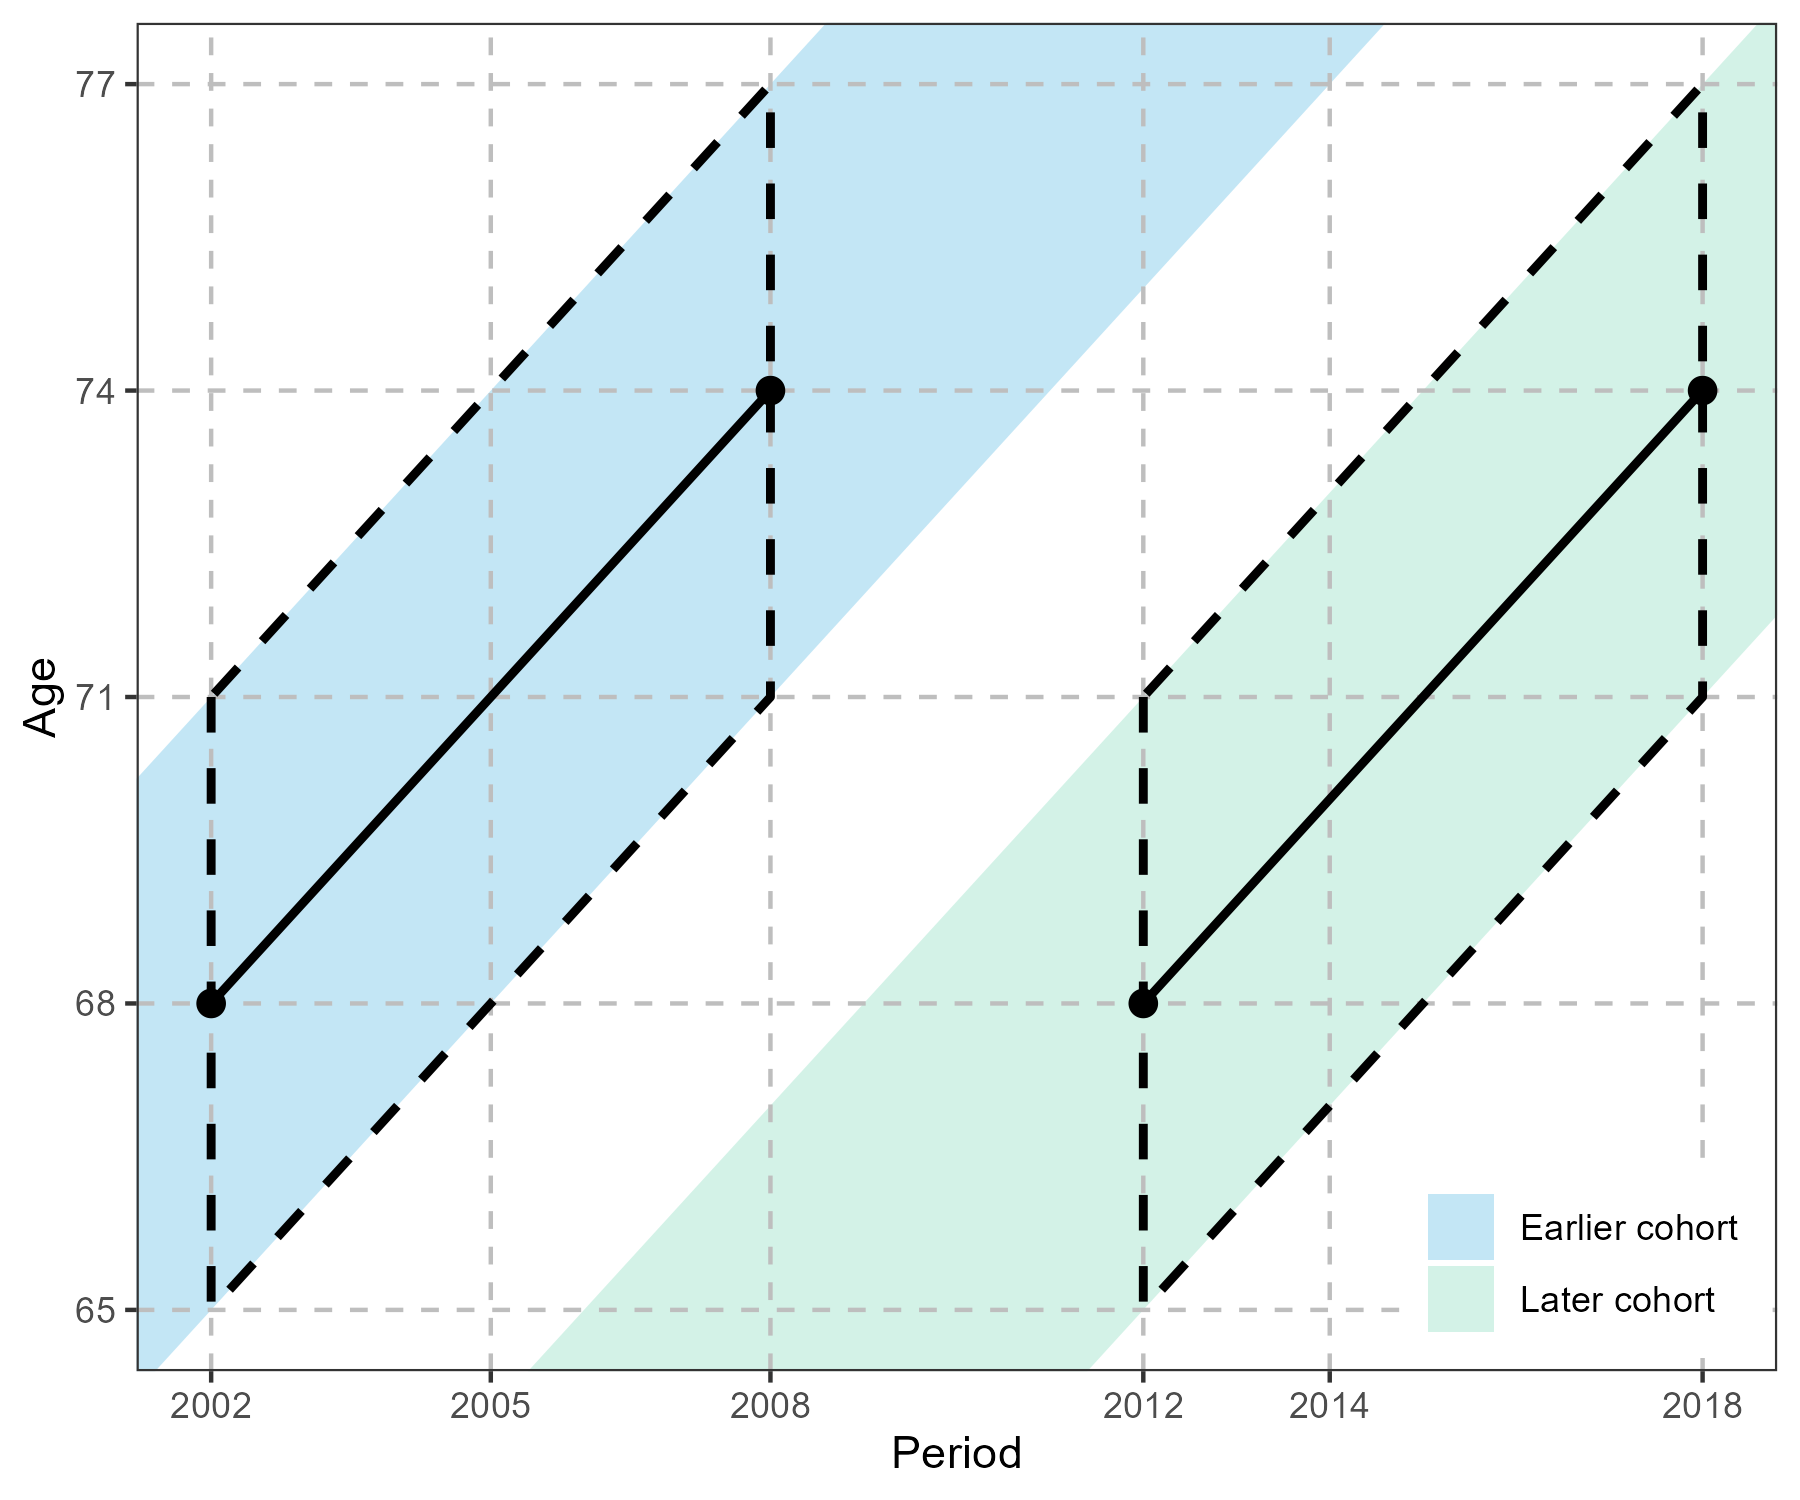
\includegraphics[width=0.8\textwidth]{fig_tabs/2_1_Lexis_Diagram.png}
  \caption{Lexis diagram used for cohort comparisons in the 68-73 age group}
  \label{fig:Lexis_Diagram}
\end{figure}

This study applied the MSLT method to estimate PC-LE and PC-HapLE. As shown in Figure 2, three discrete states were defined: happy, unhappy, and dead. Four potential transitions were considered: happy to unhappy, unhappy to happy, happy to dead, and unhappy to dead. The estimation of MSLT functions was performed using the Stochastic Population Analysis for Complex Events (SPACE) program \autocite{cai.2010.estimation} in SAS 9.4.

The SPACE computation process consisted of three sequential steps. First, data preprocessing was conducted to accommodate the varying intervals between CLHLS survey waves. SPACE converted CLHLS data into person-years format and imputed annual state values, filling missing years with pseudo-data to represent consecutive years of observation. Second, annual transition probabilities were estimated for each age group using multinomial logistic regression. The base model incorporated age, sex, cohort, and their two-way interaction terms to generate transition probability matrices stratified by these demographic variables. Two additional models were fitted to examine subgroup differences: one incorporating education level and another including urban-rural residence, both with interaction terms between the added variable and age, sex, and cohort. Third, microsimulation was employed to compute PC-LE and PC-HapLE based on the estimated transition probability matrices. A synthetic cohort of 100,000 individuals was created, with each person assigned an initial happiness state according to the weighted distribution observed at the starting age of each age group. Annual transitions were simulated by comparing random uniform numbers against age-specific transition probabilities until individuals reached the upper bound of their respective age range. PC-LE was calculated as the mean survival years within the age range, while PC-HapLE represented the mean years spent in the happy state. Confidence intervals were derived through bootstrap resampling with 300 iterations to capture uncertainty in both parameter estimation and microsimulation processes.

% === Figure 2 ===
\begin{figure}[htbp]
  \centering
  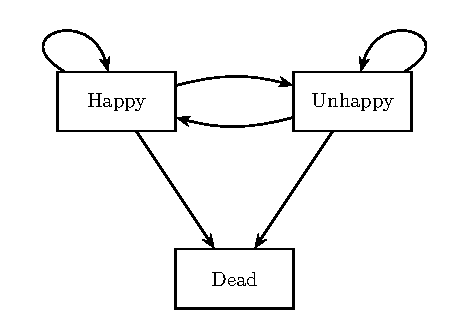
\includegraphics[width=0.8\textwidth]{fig_tabs/State_space.pdf}
  \caption{State space in the multi-state model}
  \label{fig:State_space}
\end{figure}

Inverse probability weighting (IPW) was applied to adjust for potential biases arising from differential loss to follow-up. This method assigned higher weights to individuals who completed follow-up, where weights were inversely proportional to the probability of completing follow-up. The probability models included all sociodemographic and a disability variable measured by Activities of Daily Living (ADL). IPW weights were estimated separately for each period and birth cohort, and the final analytical weight was derived by multiplying the IPW weight by the combined respondent weight from CLHLS \autocite{dugoff.2014.generalizing,liu.2019.are}.

%-------------------------------------------
% Results
%-------------------------------------------
\section{Results}
Table S1 in the Appendix presents the baseline characteristics of each birth cohort within the four age ranges examined in this study. Gender distribution remained relatively stable across cohorts within each age group, with men comprising approximately 50\%-56\% of each cohort. There is a clear trend of increasing educational attainment across cohorts within most age groups, with the proportion of literate individuals rising notably from earlier to later cohorts in the 68-73 age range (57.6\% to 72.7\%), 74-79 age range (49.3\% to 60.2\%), and 80-85 age range (43.6\% to 48.0\%). No consistent patterns are apparent in urban-rural residence distribution, which varied across cohorts within age groups. Within each age range, later cohorts generally showed higher proportions of individuals reporting happiness, with increases ranging from 1.9 to 2.9 percentage points across most age groups.

% === 3.1 ===
\subsection{Overall Cohort Differences in PC-LE and PC-HapLE}

Figure 3 and the Appendix Table S2 present estimated partial-cohort life expectancy (PC-LE), partial-cohort happy life expectancy (PC-HapLE), and partial-cohort unhappy life expectancy (PC-UnHapLE) across birth cohorts for four age ranges (68–73, 74–79, 80–85, and 86–91). Overall, later-born cohorts of Chinese older adults experienced significant increases in both the absolute number and relative proportion of happy years, accompanied by a compression of unhappy years.

Across all age ranges examined, PC-HapLE increased substantially between earlier and later cohorts. The most pronounced gains were observed in the 68–73 age range, where PC-HapLE rose 0.60 years, though this difference approached but did not reach statistical significance (95\% CI: -0.00, 1.21; p>0.05). In the 74–79 age range, the increase was statistically significant, with PC-HapLE rising by 0.40 years (95\% CI: 0.15, 0.65; p<0.01). Similar significant patterns emerged in older age ranges: 0.52 years in ages 80–85 (95\% CI: 0.23, 0.81; p<0.001) and 0.47 years in ages 86–91 (95\% CI: 0.21, 0.73; p<0.001). Concurrently, PC-UnHapLE decreased significantly across all age ranges where PC-HapLE gains were observed. The proportion of partial life expectancy spent in happiness (HapLE\%) increased substantially across cohorts, with gains ranging from 7.1 percentage points in ages 74–79 (p<0.01) to 11.5 percentage points in ages 68–73 (p<0.05). Notably, total PC-LE showed minimal change across cohorts in most age groups, with only the oldest age range 86-91 showing a statistically significant increase of 0.21 years (95\% CI: 0.04, 0.37; p<0.05).

% === Figure 3 ===
\begin{figure}[!p]
  \centering
  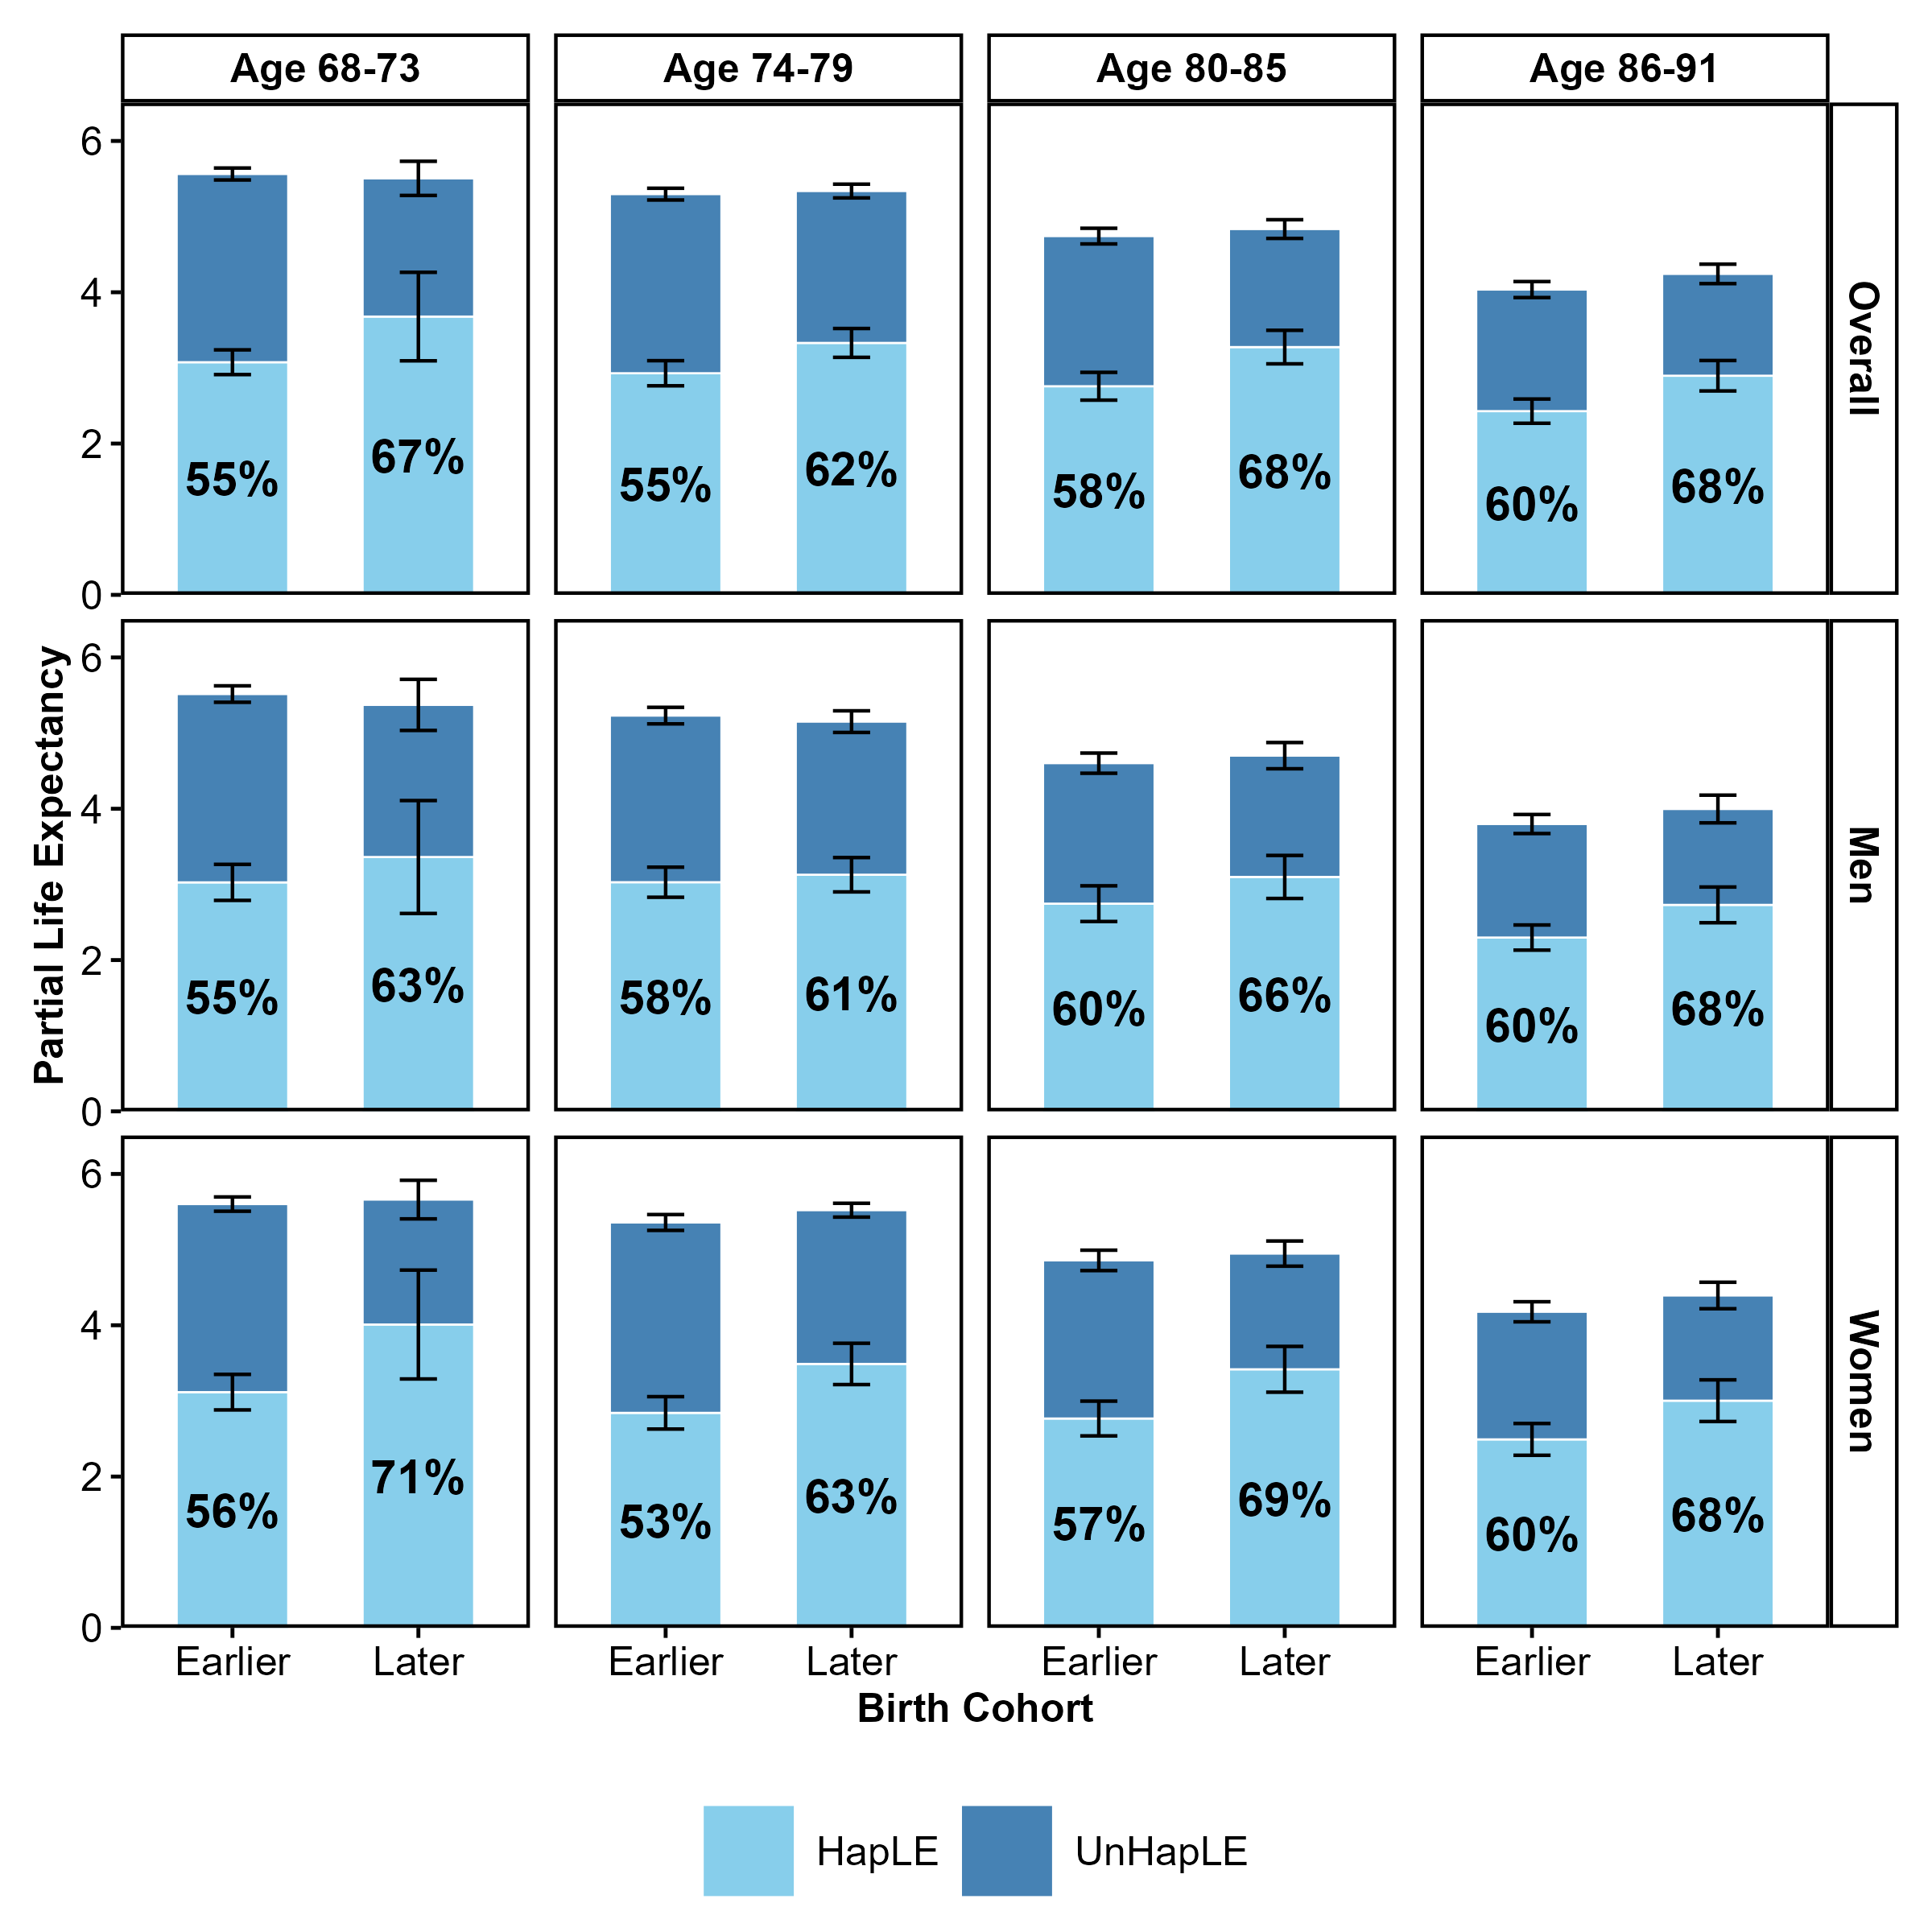
\includegraphics[width=1\textwidth]{fig_tabs/2_2_HapLE_stacked_plots_sex.png}
  \caption{Estimated PC-LE, PC-HapLE and PC-UnHapLE across birth cohorts by age range and sex. The black vertical lines denote the 95\% CI around each point estimate. The percentage figure in each bar shows HapLE\%.}
\end{figure}

% === 3.2 ===
\subsection{Cohort Differences in PC-LE and PC-HapLE by Gender}

Figure 3 and Table S2 also show substantial gender disparities in cohort changes of PC-HapLE. Older women experienced consistently larger and more statistically significant improvements in PC-HapLE compared to men across most age ranges.

Among women, significant increases in PC-HapLE were observed in all four age groups examined: 0.89 years in ages 68–73 (95\% CI: 0.14, 1.65; p<0.05), 0.65 years in ages 74–79 (95\% CI: 0.30, 0.99; p<0.001), 0.65 years in ages 80–85 (95\% CI: 0.27, 1.03; p<0.001), and 0.51 years in ages 86–91 (95\% CI: 0.17, 0.86; p<0.01). In contrast, men showed more modest and less consistent gains. A statistically significant increase in PC-HapLE among men was observed only in the oldest age group (86–91), with a gain of 0.43 years (95\% CI: 0.14, 0.72; p<0.01). For other age groups, while point estimates suggested modest improvements, the wide confidence intervals indicated considerable uncertainty around these estimates, and the changes did not reach statistical significance. These patterns resulted in larger proportional gains in HapLE\% for women, with increases ranging from 8.7 to 15.2 percentage points across age groups, compared to more modest gains for men.

% === 3.3 ===
\subsection{Cohort Differences in PC-LE and PC-HapLE by Education}

As detailed in Figure 4 and the Appendix Table S3, there were significant differences in PC-HapLE between literate and illiterate older adults across most age ranges. Literate older adults consistently experienced larger and more statistically significant gains in PC-HapLE compared to their illiterate counterparts across most age ranges examined.

Among literate older adults, significant increases in PC-HapLE were observed in three age groups: 0.58 years in ages 68–73 (95\% CI: -0.06, 1.21; approaching significance), 0.47 years in ages 74–79 (95\% CI: 0.15, 0.79; p<0.01), 0.70 years in ages 80–85 (95\% CI: 0.26, 1.13; p<0.01), and 0.70 years in ages 86–91 (95\% CI: 0.22, 1.18; p<0.01). These improvements were accompanied by substantial increases in HapLE\%, particularly notable in ages 80–85 where the proportion rose by 13.9 percentage points (p<0.001). In contrast, illiterate older adults showed smaller and less consistent improvements. Statistically significant gains in PC-HapLE were observed only in the oldest age group (86–91), with an increase of 0.35 years (95\% CI: 0.06, 0.63; p<0.05). For other age groups, while point estimates suggested modest improvements, the differences were not statistically significant.

% === Figure 4 ===
\begin{figure}[!p]
  \centering
  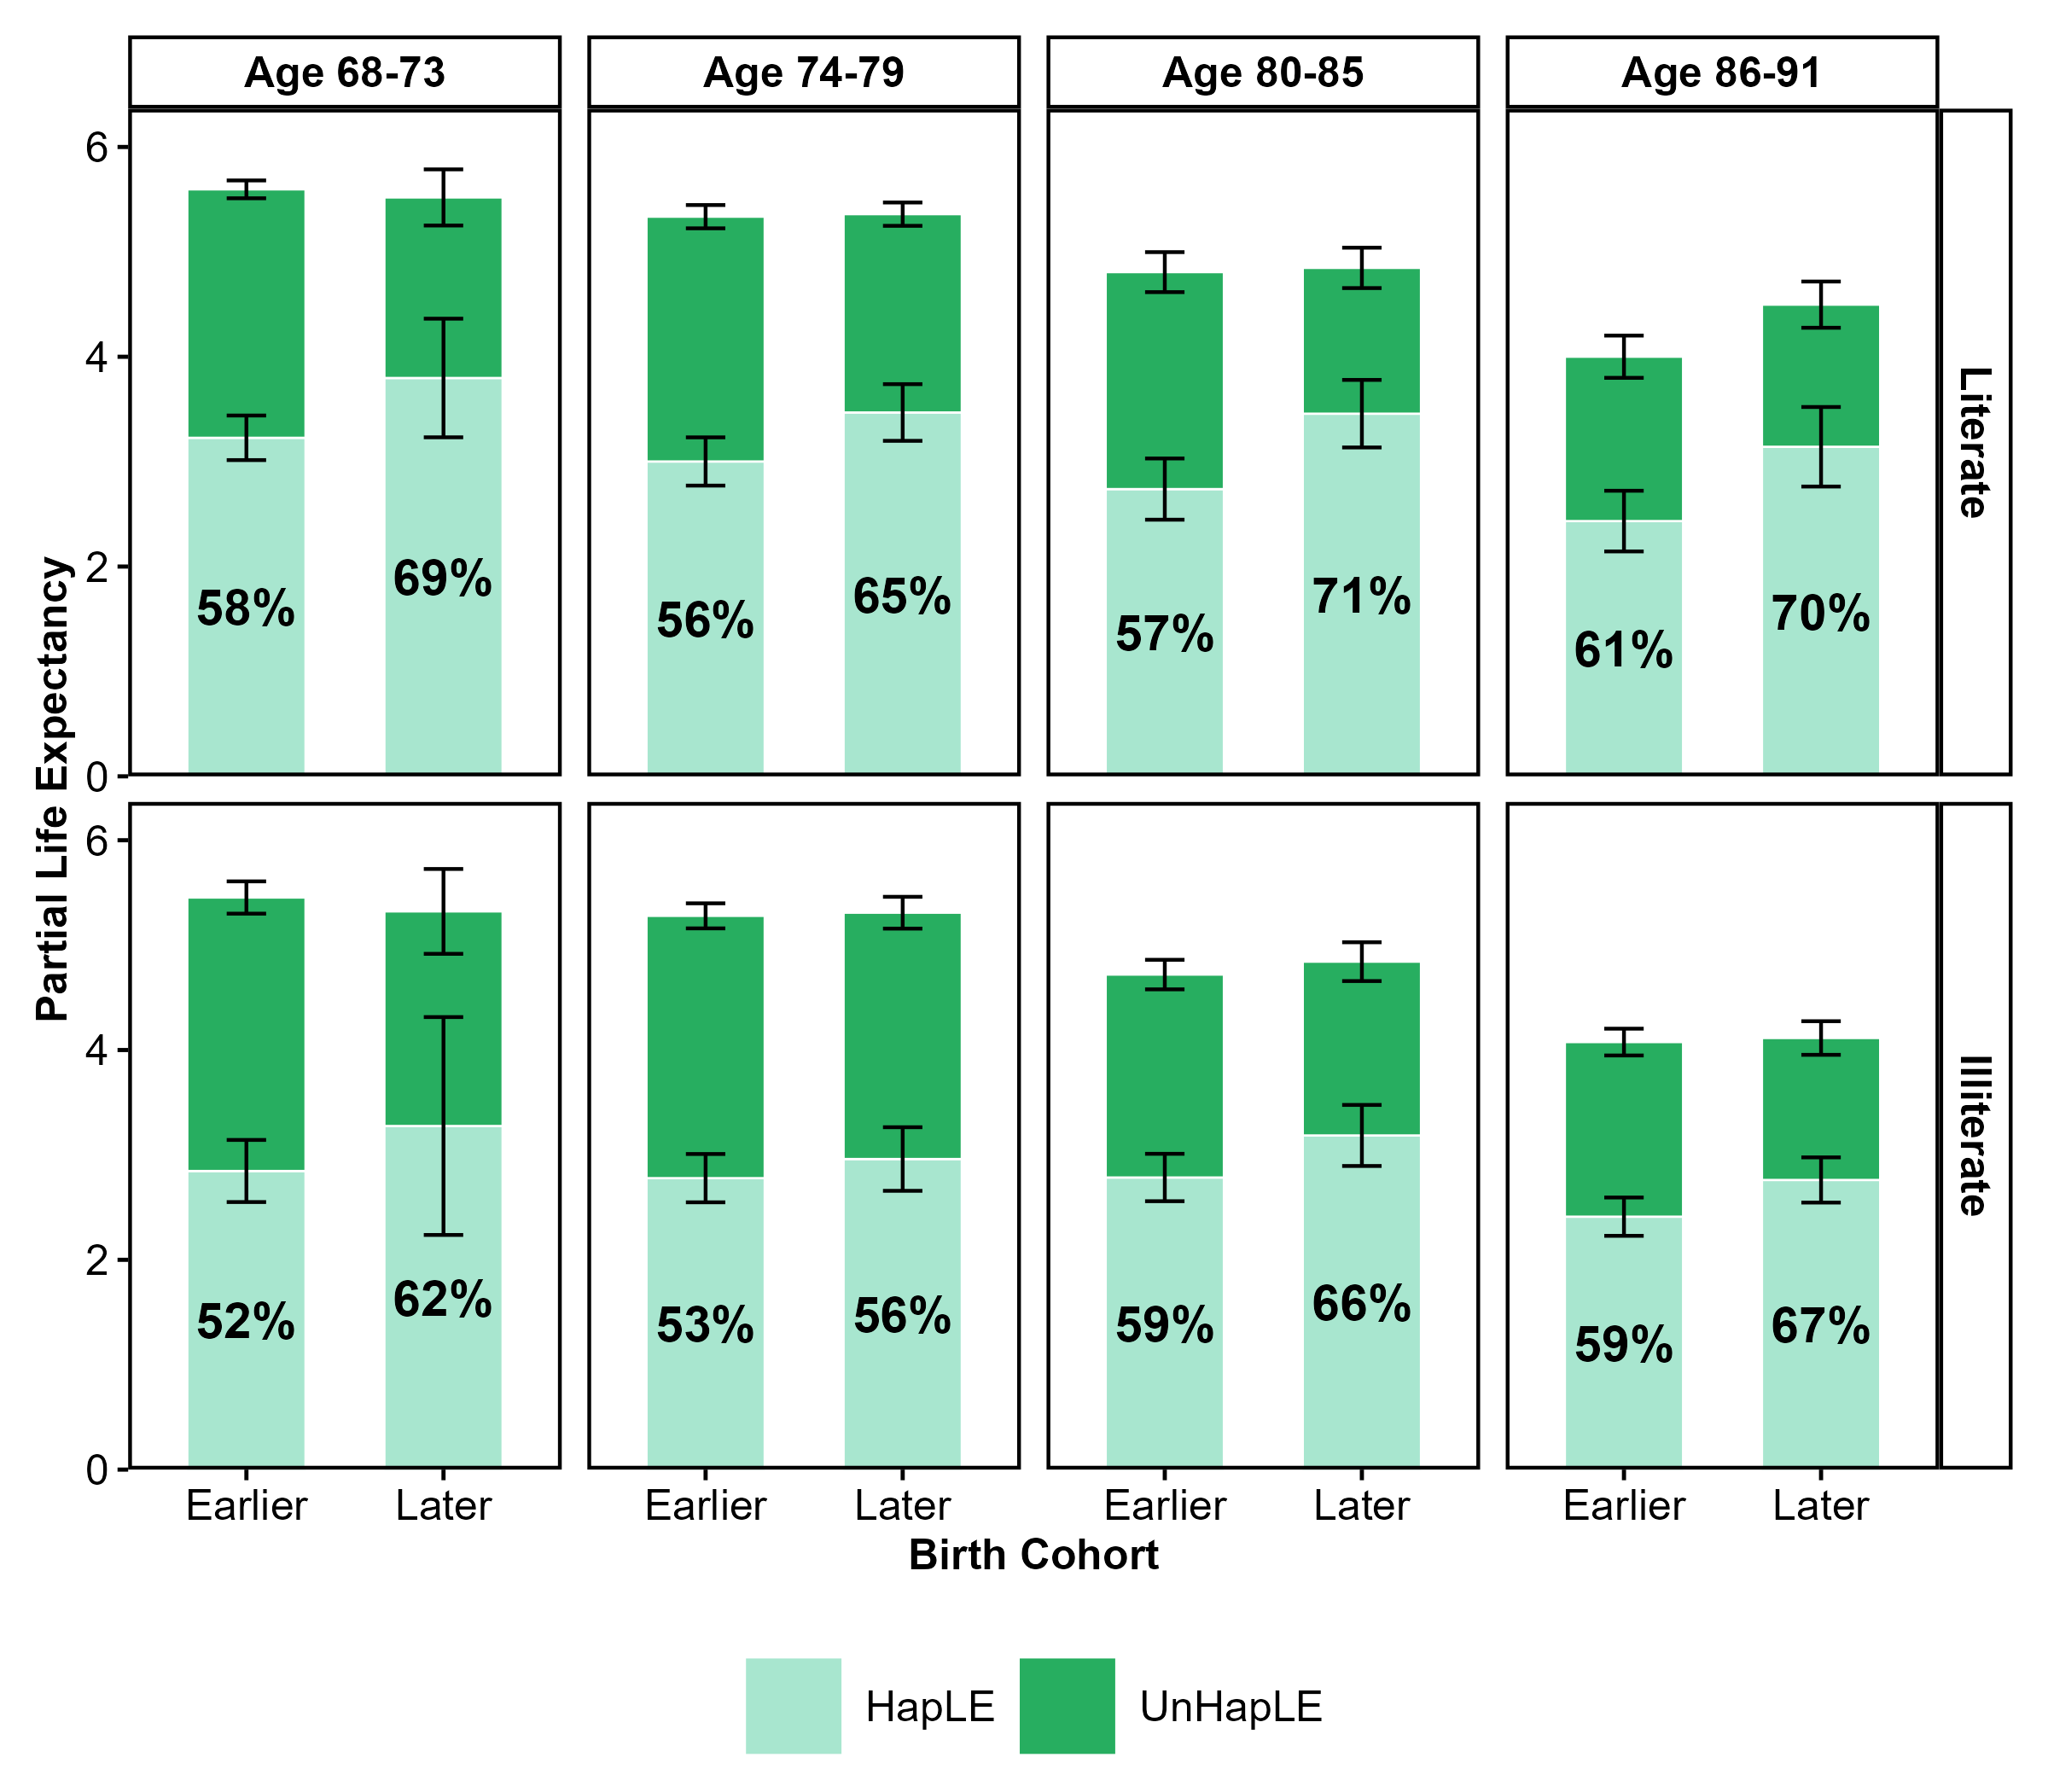
\includegraphics[width=1\textwidth]{fig_tabs/2_3_HapLE_stacked_plots_edu.png}
  \caption{Estimated PC-LE, PC-HapLE and PC-UnHapLE across birth cohorts by age range and education. The black vertical lines denote the 95\% CI around each point estimate. The percentage figure in each bar shows HapLE\%.}
\end{figure}

% === 3.4 ===
\subsection{Cohort Differences in PC-LE and PC-HapLE by Residence}

The most pronounced disparities in cohort trends were observed between urban and rural residents (Figure 5 and the Appendix Table S4). Urban older adults experienced substantial and highly significant improvements in PC-HapLE and HapLE\% across all age groups, while rural residents showed more modest and inconsistent gains.

Among urban residents, significant increases in PC-HapLE were observed across all four age ranges: 1.05 years in ages 68–73 (95\% CI: 0.45, 1.64; p<0.001), 0.51 years in ages 74–79 (95\% CI: 0.19, 0.83; p<0.01), 0.56 years in ages 80–85 (95\% CI: 0.21, 0.91; p<0.01), and 0.45 years in ages 86–91 (95\% CI: 0.14, 0.77; p<0.01). These improvements were accompanied by dramatic increases in HapLE\%, most notably in ages 68–73 where the proportion increased by 17.0 percentage points (p<0.01). Rural residents showed a markedly different pattern. Statistically significant increases in PC-HapLE were observed only in the two oldest age groups: 0.43 years in ages 80–85 (95\% CI: 0.05, 0.81; p<0.05) and 0.45 years in ages 86–91 (95\% CI: 0.11, 0.79; p<0.01). In the younger age groups (68–73 and 74–79), while point estimates suggested modest improvements, the differences were not statistically significant.

% === Figure 5 ===
\begin{figure}[!p]
  \centering
  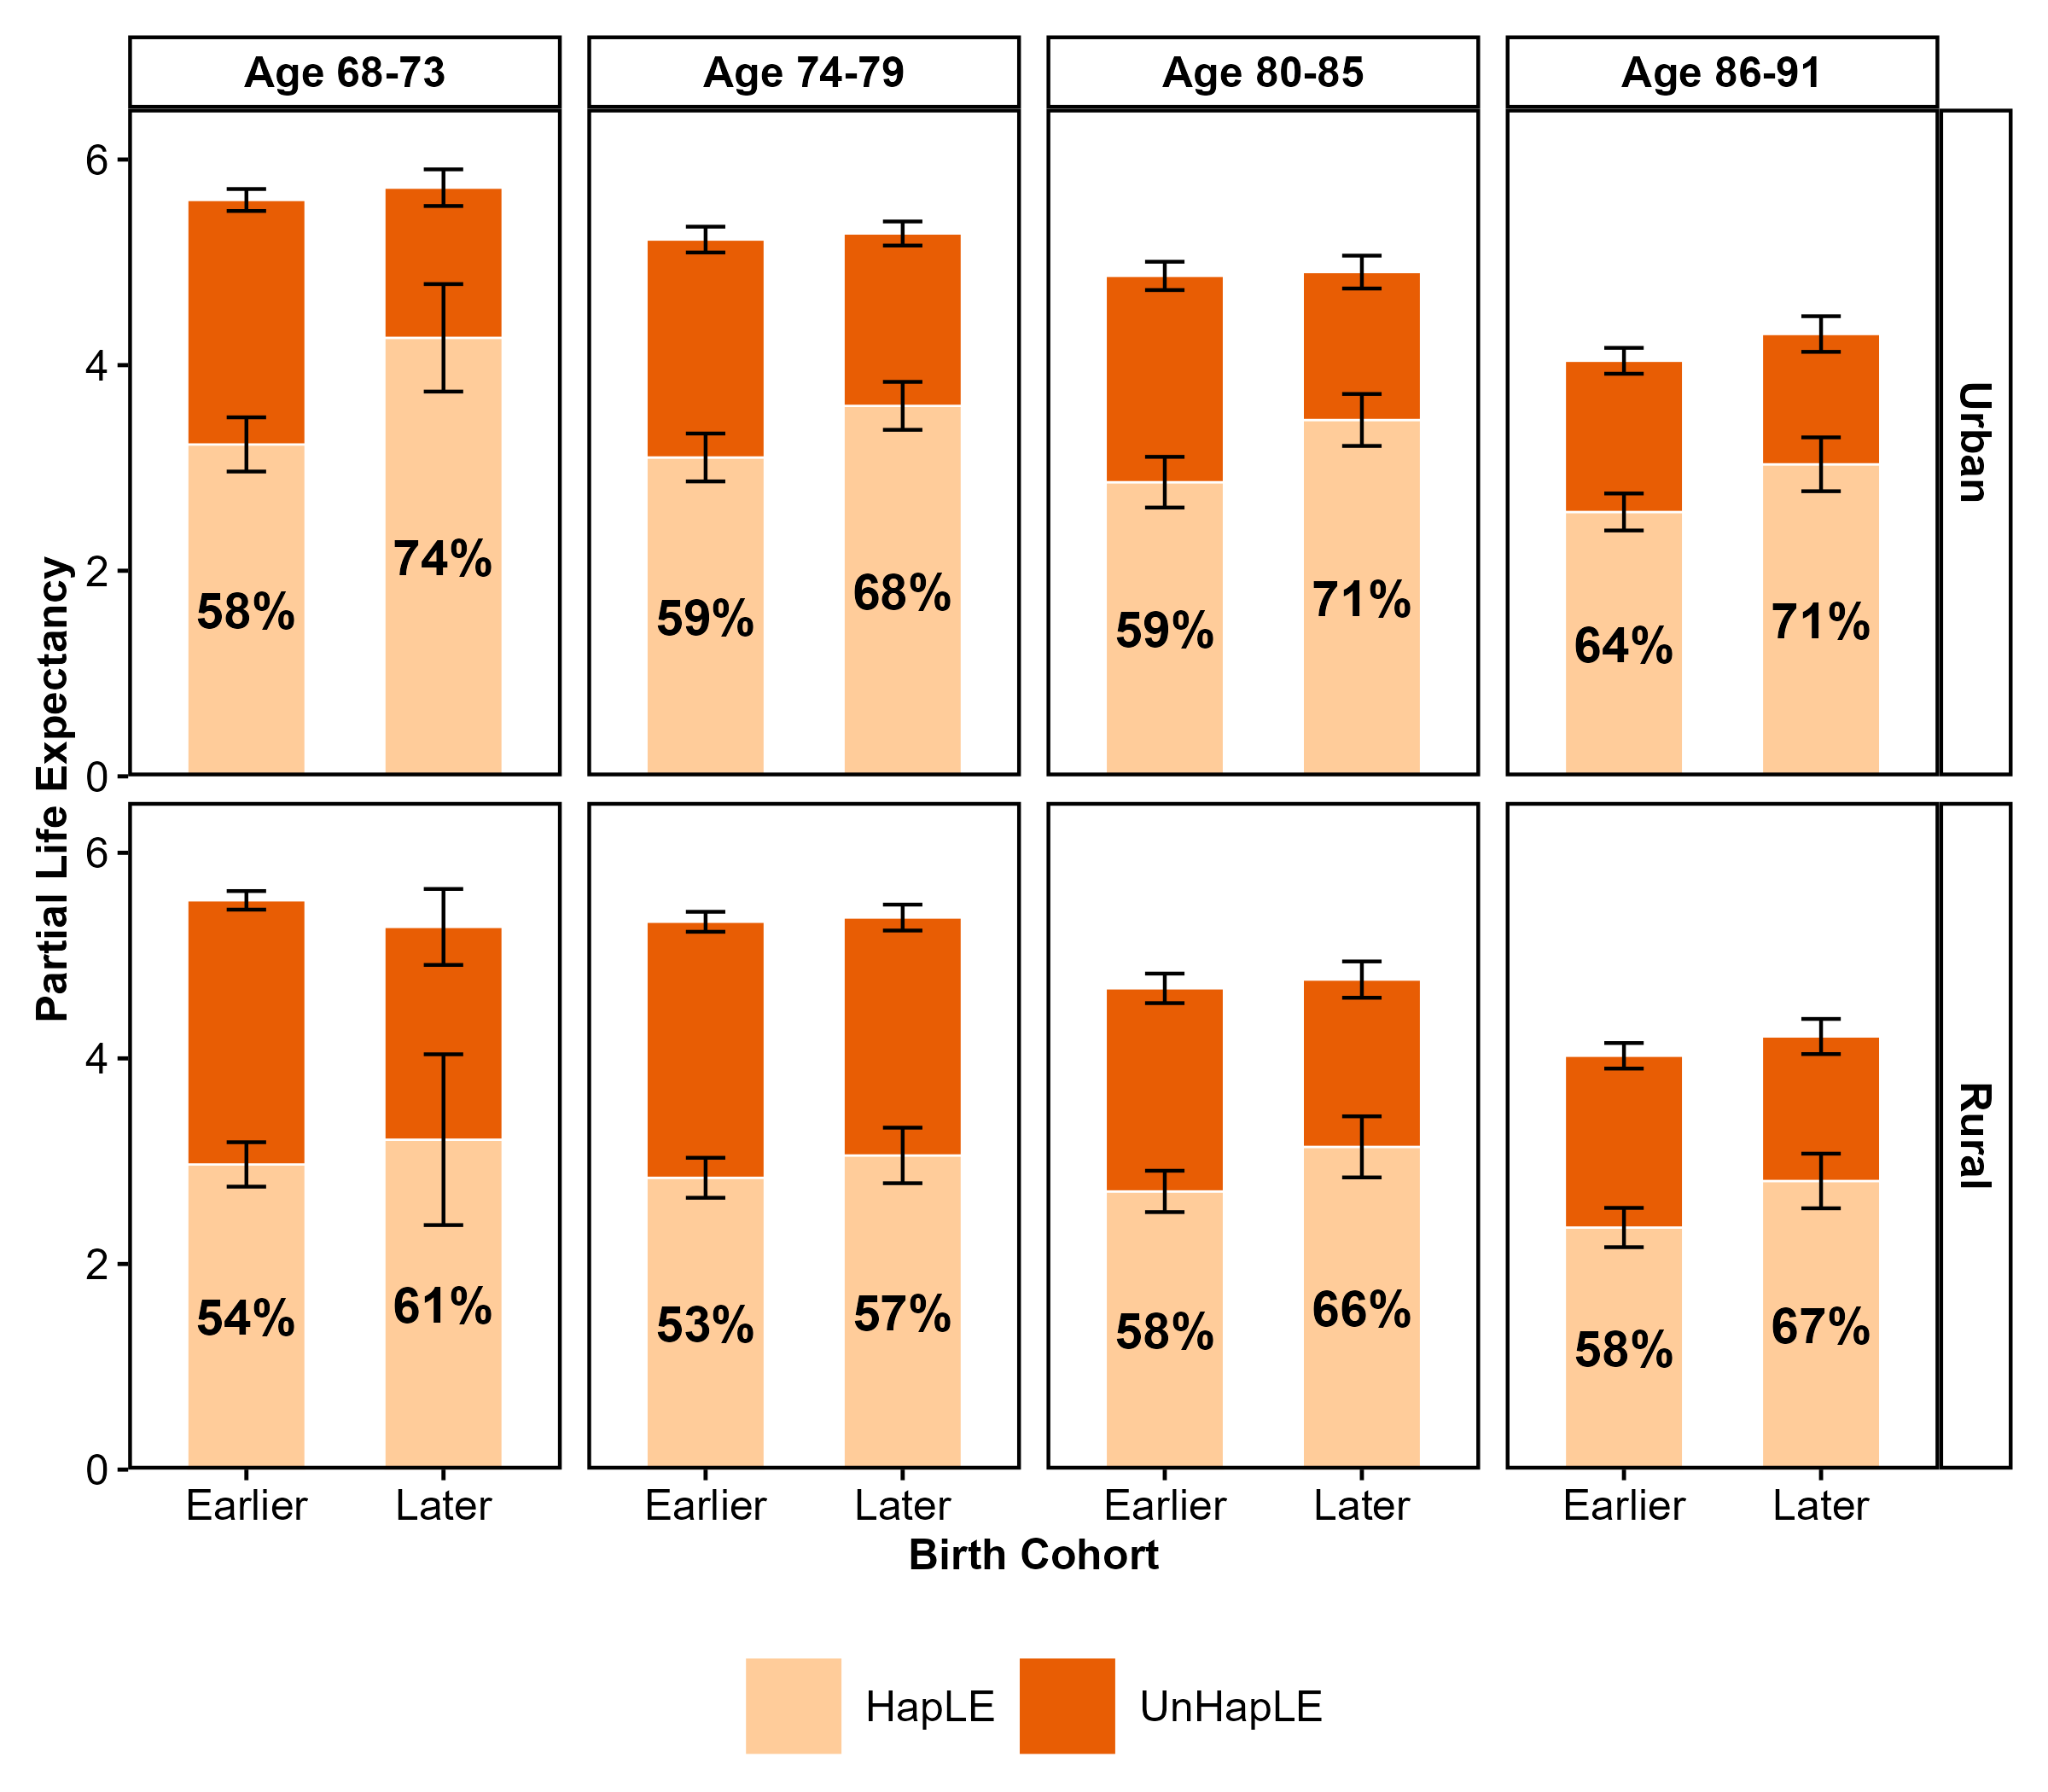
\includegraphics[width=1\textwidth]{fig_tabs/2_4_HapLE_stacked_plots_urban.png}
  \caption{Estimated PC-LE, PC-HapLE and PC-UnHapLE across birth cohorts by age range and residence. The black vertical lines denote the 95\% CI around each point estimate. The percentage figure in each bar shows HapLE\%.}
\end{figure}

%-------------------------------------------
% Discussion
%-------------------------------------------
\section{Discussion}

Using the national representative longitudinal data and a cohort-based multi-state life table approach, this study provides novel evidence to address the question of whether older adults in China are living longer happy years. Our findings reveal a significant and positive trend: later-born cohorts, across all examined age ranges from 68 to 91, are expected to live a greater number of years in a happy state and a higher proportion of their remaining life in happiness compared to their earlier-born counterparts. This gain in happy years was primarily achieved through a "compression of unhappiness"—a notable reduction in the expected years lived in an unhappy state—while total partial-cohort life expectancy remained largely stable across most age groups. However, this optimistic aggregate trend masks profound and widening disparities. The gains in happy years were not equitably distributed, with improvements being substantially larger for women, literate individuals, and especially urban residents, suggesting that the benefits of socioeconomic progress have disproportionately favored more advantaged subgroups.

The observed "compression of unhappiness" across birth cohorts extends previous research and offers a cohort-based perspective on a widely debated topic in China. Our finding  is consistent with the period-based analysis by Duan and Chen \autocite{duan.2020.happy}, who also documented an "unhappiness compression" pattern in the general adult population. Our use of a cohort design provides stronger evidence that this is a generational phenomenon rather than a simple period effect \autocite{payne.2022.expansion}. This optimistic cohort trend also offers a nuanced counterpoint to the "Easterlin paradox," which posited that China’s rapid economic growth during the 1990s and early 2000s did not uniformly translate into greater life satisfaction \autocite{easterlin.2012.chinas}. Our results align more closely with recent studies indicating that Chinese happiness levels have been rising since the early 2000s, as the benefits of development became more widespread \autocite{wang.2023.hierarchical,cai.2023.does}. Several key factors likely contributed to the observed gains in happy life expectancy across the cohorts in our study. The observation periods of our analysis coincide with a period of maturation in China's social and economic systems. The older adults in our study were direct beneficiaries of the substantial expansion and consolidation of China's social security programs. The nationwide rollout of near-universal pension systems and health insurance schemes, including the New Rural Cooperative Medical System and the Urban Resident Basic Medical Insurance, provided a crucial buffer against economic and health-related shocks \autocite{liu.2019.are}. This enhanced security, alongside improvements in public infrastructure and the continued, albeit changing, role of family support, has likely contributed to a more favorable environment for well-being in later life.

An interesting finding is the significant gender disparity in cohort differences, with older women experiencing substantially larger and more consistent gains in happy life expectancy (HapLE) than men. This finding contrasts with previous period-based evidence from China, which suggested that while women had a longer HapLE, this advantage was primarily driven by their lower mortality rather than a higher prevalence of happiness in later life \autocite{duan.2020.happy}. Our study reveals a fundamental shift: the gains in HapLE for women are driven by a “compression of unhappiness,” indicating an improvement in the quality, not just the quantity, of later-life years. One possible explanation for this phenomenon is that the trend is driven less by women’s objective conditions improving faster than men’s (the composition effect), and more by women deriving greater subjective well-being from the same life improvements (the coefficient effect) \autocite{yang.2024.gender}. Furthermore, women’s deeper embeddedness in family and community life means they likely gained more from improvements in community environments and social support systems, which are central to their daily routines and well-being \autocite{feng.2024.gender}.

Perhaps the most critical finding of this study is the widening socioeconomic gap in happy life expectancy, particularly between urban and rural residents. While previous research confirmed static inequalities at a single time point \autocite{wan.2024.socioeconomic}, our cohort analysis reveals a more troubling dynamic: the disparity is actively growing, creating a deepening "happiness gap." This growing urban-rural divide is likely rooted in China's dualistic socioeconomic structure, which has long favored urban areas in resource allocation. Urban older adults have consistently benefited from more generous pensions, higher-quality healthcare, and better-developed community infrastructure \autocite{liu.2019.are}. Although rural social security has improved, the level of protection remains substantially lower, leaving rural older adults less able to translate national development into personal well-being. Similarly, the education gap reflects disparities in the capacity to leverage resources. As a key determinant of socioeconomic status \autocite{payne.2022.expansion,shen.2023.disability}, education equips individuals to better navigate complex healthcare and social welfare systems, an advantage that allows them to more effectively convert available opportunities into longer and happier lives \autocite{wan.2024.socioeconomic}. It is important to acknowledge that these two dimensions of inequality were analyzed in separate models due to the limitation of sample size. Given that urban populations in China are, on average, more educated, the effects we attribute to each factor are not fully disentangled. However, the fact that both show an independent predictive effect underscores that socioeconomic disadvantage is a multifaceted force. This suggests that while intertwined, the structural resource disparities and differences in individual capacity driving these gaps represent distinct mechanisms that warrant separate consideration.

Several limitations should be considered when interpreting the findings. First, our measurement of happiness relies on a single-item life satisfaction question, which, although widely validated and used in large-scale surveys, cannot capture the full multidimensional nature of well-being \autocite{george.2010.still}. Additionally, the dichotomization of the five-point scale into "happy" and "unhappy" categories, while facilitating model estimation, may result in a loss of information about the gradual differences in satisfaction levels \autocite{wan.2024.socioeconomic}. Second, our analysis focuses on partial-cohort happy life expectancy within bounded age ranges rather than complete life-course measures. While this approach enables the examination of living cohorts, the results should not be directly extrapolated to full lifetime happiness trajectories, particularly given the potential for major social or policy disruptions that could alter later-life patterns \autocite{payne.2022.expansion}. Third, the multistate life table model employed in this study is based on a first-order Markov assumption, meaning that happiness transitions depend only on the current state and not on the duration spent in that state or past emotional trajectories. This simplifies the complex psychological dynamics of well-being in reality \autocite{payne.2022.expansion,shen.2023.disability}. Related to this, the panel nature of CLHLS data, with surveys conducted every three or four years, assumes only annual transitions between waves, potentially missing short-term fluctuations or multiple transitions in happiness states that may occur between survey periods.

One of the main strengths of this study is its focus on understanding changes in happy life expectancy across birth cohorts, rather than relying solely on period-based comparisons. Though period-based approach may be useful for monitoring aggregate trends in population-level happiness, these results do not easily translate to the experience of any given cohort of individuals \autocite{payne.2022.expansion}. Our cohort-based approach provides results that match more closely with the lived experience of individuals within the population and offers clearer insights into generational changes in happy longevity. A second strength lies in our comprehensive examination of socioeconomic disparities in HapLE trends. While previous studies have documented static inequalities in HapLE at single time points \autocite{wan.2024.socioeconomic}, our analysis reveals the dynamic patterns of how these disparities evolve across cohorts, thus providing new evidence on whether the benefits of China's socioeconomic development are being equitably distributed across different population subgroups. Additionally, our analysis uses CLHLS, one of the largest and most comprehensive longitudinal datasets of older adults worldwide, providing a unique opportunity to examine happiness trajectories among a substantial portion of the global aging population. The combination of this data source with the multistate life table method enables robust estimation of HapLE across cohorts and subgroups, supporting the reliability and generalizability of our findings.
%-------------------------------------------
% Conclusion
%-------------------------------------------
\section{Conclusion}

In conclusion, this study provides evidence that older adults in China are indeed living longer happy years across generations, largely driven by a significant "compression of unhappiness" rather than an extension of total lifespan. This optimistic aggregate trend, however, conceals a crucial and troubling counter-narrative: the profound widening of a "happiness gap." The benefits of China's rapid socioeconomic development have not been equitably distributed, disproportionately favoring urban, educated, and female older adults. While these advantaged groups are experiencing accelerated gains in happiness, their rural and less-educated counterparts are being left behind, creating a deepening divide in the quality of later life. These findings challenge policymakers to look beyond extending longevity and to urgently address the structural inequalities that prevent the gains of national progress from translating into universal well-being. To foster a truly equitable aging society, future policy must pivot from simply adding years to life, to ensuring that those added years are happy ones for all.

%-------------------------------------------
% References
%-------------------------------------------
\newpage
\printbibliography

%-------------------------------------------
% Appendix
%-------------------------------------------
\renewcommand\theequation{\Alph{section}\arabic{equation}} %Redefine equation numbering format
\counterwithin*{equation}{section} % Number equations within sections
\renewcommand\thefigure{\Alph{section}\arabic{figure}} % Redefine equation numbering format
\counterwithin*{figure}{section} % Number equations within sections
% Manual table numbering for supplementary tables (S1, S2, S3, S4)

\newpage
\begin{appendices}

  \section*{Appendix}

  % === Table S1: Descriptive Table ===
  \vspace*{\fill}
  \begin{table}[!h]
    \centering
    \caption*{\textbf{Table S1.} Descriptive statistics of the sample by age range and cohort}
    \label{tab:S1_desc_stats}
    \resizebox{\ifdim\width>\linewidth\linewidth\else\width\fi}{!}{%
      \begin{tabular}{lcccccccc}
        \toprule
        \textbf{Age Range} & \multicolumn{2}{c}{\textbf{68--73}} & \multicolumn{2}{c}{\textbf{74--79}} & \multicolumn{2}{c}{\textbf{80--85}} & \multicolumn{2}{c}{\textbf{86--91}}                                                                                 \\
        \cmidrule(lr){2-3} \cmidrule(lr){4-5} \cmidrule(lr){6-7} \cmidrule(lr){8-9}
        \textbf{Cohort}    & \textbf{1932--37}                   & \textbf{1942--47}                   & \textbf{1926--31}                   & \textbf{1936--41}                   & \textbf{1920--25} & \textbf{1930--35} & \textbf{1914--19} & \textbf{1924--29} \\
        \midrule
        \textbf{N}         & 1643                                & 754                                 & 1677                                & 1370                                & 1763              & 1194              & 1288              & 903               \\
        \midrule
        \textbf{Gender (\%)}                                                                                                                                                                                                                                       \\
        \quad Men          & 51.7                                & 56.0                                & 50.4                                & 53.2                                & 51.4              & 51.8              & 53.3              & 52.9              \\
        \quad Women        & 48.3                                & 44.0                                & 49.6                                & 46.8                                & 48.6              & 48.2              & 46.7              & 47.1              \\
        \midrule
        \textbf{Education (\%)}                                                                                                                                                                                                                                    \\
        \quad Literate     & 57.6                                & 72.7                                & 49.3                                & 60.2                                & 43.6              & 48.0              & 46.6              & 40.4              \\
        \quad Illiterate   & 42.4                                & 27.3                                & 50.7                                & 39.8                                & 56.4              & 52.0              & 53.4              & 59.6              \\
        \midrule
        \textbf{Residence (\%)}                                                                                                                                                                                                                                    \\
        \quad Urban        & 41.3                                & 41.9                                & 40.9                                & 51.0                                & 43.4              & 49.8              & 51.0              & 46.6              \\
        \quad Rural        & 58.7                                & 58.1                                & 59.1                                & 49.0                                & 56.6              & 50.2              & 49.0              & 53.4              \\
        \midrule
        \textbf{Happiness (\%)}                                                                                                                                                                                                                                    \\
        \quad Happy        & 56.7                                & 58.6                                & 57.1                                & 56.9                                & 58.4              & 60.1              & 59.1              & 56.0              \\
        \quad Unhappy      & 43.3                                & 41.4                                & 42.9                                & 43.1                                & 41.6              & 39.9              & 40.9              & 44.0              \\
        \midrule
        \textbf{Disability (\%)}                                                                                                                                                                                                                                   \\
        \quad 0 ADL        & 96.3                                & 95.8                                & 93.4                                & 92.8                                & 86.2              & 88.4              & 77.3              & 82.2              \\
        \quad 1+ ADL       & 3.7                                 & 4.2                                 & 6.6                                 & 7.2                                 & 13.8              & 11.6              & 22.7              & 17.8              \\
        \bottomrule
      \end{tabular}%
    }
  \end{table}
  \vspace*{\fill}

  % === Table S2 ===
  \vspace*{\fill}
  \begin{table}[!p]
    \centering
    \caption*{\textbf{Table S2.} Estimated PC-LE, PC-HapLE, PC-UnHapLE, HapLE\% and UnHapLE\% and their differences across birth cohorts by age range and sex. The differences were calculated as the difference between the later cohort and the earlier cohort. The 95\% CI around each point estimate is shown in parentheses. Significance of difference: * p$<$0.05, ** p$<$0.01, *** p$<$0.001.}
    \centering
    \resizebox{\ifdim\width>\linewidth\linewidth\else\width\fi}{!}{
      \begin{tabular}[t]{>{}l>{}lllllll}
        \toprule
        \textbf{Age Range}                    & \textbf{Sex}                    & \textbf{Cohort}               & \textbf{PC-LE}                              & \textbf{PC-HapLE}                            & \textbf{HapLE\%}                            & \textbf{PC-UnHapLE}                             & \textbf{UnHapLE\%}                             \\
        \midrule
        \multirow{9}{*}[-4ex]{\textbf{68-73}} & \multirow{3}{*}{\textbf{All}}   & Earlier                       & 5.56 (5.48, 5.64)                           & 3.08 (2.91, 3.24)                            & 55.3 (52.5, 58.1)                           & 2.49 (2.33, 2.65)                               & 44.7 (41.9, 47.5)                              \\
        \cmidrule{3-8}
                                              &                                 & Later                         & 5.51 (5.28, 5.73)                           & 3.68 (3.09, 4.26)                            & 66.8 (57.4, 76.3)                           & 1.83 (1.33, 2.32)                               & 33.2 (23.7, 42.6)                              \\
        \cmidrule{3-8}
                                              &                                 & \cellcolor{gray!10}\em{Diff.} & \cellcolor{gray!10}\em{-0.06 (-0.30, 0.18)} & \cellcolor{gray!10}\em{0.60 (-0.00, 1.21)}   & \cellcolor{gray!10}\em{11.5 (1.7, 21.4)*}   & \cellcolor{gray!10}\em{-0.66 (-1.18, -0.14)*}   & \cellcolor{gray!10}\em{-11.5 (-21.4, -1.7)*}   \\
        \cmidrule{2-8}
                                              & \multirow{3}{*}{\textbf{Men}}   & Earlier                       & 5.52 (5.41, 5.62)                           & 3.03 (2.79, 3.27)                            & 54.9 (50.8, 58.9)                           & 2.49 (2.27, 2.71)                               & 45.1 (41.1, 49.2)                              \\
        \cmidrule{3-8}
                                              &                                 & Later                         & 5.37 (5.04, 5.71)                           & 3.36 (2.62, 4.11)                            & 62.6 (50.3, 74.9)                           & 2.01 (1.36, 2.66)                               & 37.4 (25.1, 49.7)                              \\
        \cmidrule{3-8}
                                              &                                 & \cellcolor{gray!10}\em{Diff.} & \cellcolor{gray!10}\em{-0.14 (-0.50, 0.21)} & \cellcolor{gray!10}\em{0.34 (-0.45, 1.12)}   & \cellcolor{gray!10}\em{7.7 (-5.2, 20.6)}    & \cellcolor{gray!10}\em{-0.48 (-1.16, 0.21)}     & \cellcolor{gray!10}\em{-7.7 (-20.6, 5.2)}      \\
        \cmidrule{2-8}
                                              & \multirow{3}{*}{\textbf{Women}} & Earlier                       & 5.60 (5.51, 5.70)                           & 3.12 (2.88, 3.35)                            & 55.6 (51.4, 59.8)                           & 2.49 (2.24, 2.73)                               & 44.4 (40.2, 48.6)                              \\
        \cmidrule{3-8}
                                              &                                 & Later                         & 5.66 (5.41, 5.92)                           & 4.01 (3.29, 4.73)                            & 70.8 (59.4, 82.2)                           & 1.65 (1.03, 2.27)                               & 29.2 (17.8, 40.6)                              \\
        \cmidrule{3-8}
                                              &                                 & \cellcolor{gray!10}\em{Diff.} & \cellcolor{gray!10}\em{0.06 (-0.21, 0.33)}  & \cellcolor{gray!10}\em{0.89 (0.14, 1.65)*}   & \cellcolor{gray!10}\em{15.2 (3.1, 27.3)*}   & \cellcolor{gray!10}\em{-0.83 (-1.50, -0.17)*}   & \cellcolor{gray!10}\em{-15.2 (-27.3, -3.1)*}   \\
        \cmidrule{1-8}
        \multirow{9}{*}[-4ex]{\textbf{74-79}} & \multirow{3}{*}{\textbf{All}}   & Earlier                       & 5.30 (5.22, 5.37)                           & 2.93 (2.76, 3.10)                            & 55.3 (52.3, 58.3)                           & 2.37 (2.21, 2.53)                               & 44.7 (41.7, 47.7)                              \\
        \cmidrule{3-8}
                                              &                                 & Later                         & 5.34 (5.25, 5.43)                           & 3.33 (3.14, 3.52)                            & 62.4 (58.9, 65.9)                           & 2.01 (1.82, 2.20)                               & 37.6 (34.1, 41.1)                              \\
        \cmidrule{3-8}
                                              &                                 & \cellcolor{gray!10}\em{Diff.} & \cellcolor{gray!10}\em{0.04 (-0.08, 0.16)}  & \cellcolor{gray!10}\em{0.40 (0.15, 0.65)**}  & \cellcolor{gray!10}\em{7.1 (2.5, 11.7)**}   & \cellcolor{gray!10}\em{-0.36 (-0.61, -0.11)**}  & \cellcolor{gray!10}\em{-7.1 (-11.7, -2.5)**}   \\
        \cmidrule{2-8}
                                              & \multirow{3}{*}{\textbf{Men}}   & Earlier                       & 5.23 (5.12, 5.34)                           & 3.03 (2.83, 3.23)                            & 57.9 (54.3, 61.5)                           & 2.20 (2.01, 2.40)                               & 42.1 (38.5, 45.7)                              \\
        \cmidrule{3-8}
                                              &                                 & Later                         & 5.15 (5.01, 5.29)                           & 3.13 (2.90, 3.36)                            & 60.7 (56.3, 65.1)                           & 2.02 (1.78, 2.27)                               & 39.3 (34.9, 43.7)                              \\
        \cmidrule{3-8}
                                              &                                 & \cellcolor{gray!10}\em{Diff.} & \cellcolor{gray!10}\em{-0.08 (-0.26, 0.10)} & \cellcolor{gray!10}\em{0.10 (-0.20, 0.40)}   & \cellcolor{gray!10}\em{2.8 (-2.9, 8.5)}     & \cellcolor{gray!10}\em{-0.18 (-0.49, 0.13)}     & \cellcolor{gray!10}\em{-2.8 (-8.5, 2.9)}       \\
        \cmidrule{2-8}
                                              & \multirow{3}{*}{\textbf{Women}} & Earlier                       & 5.36 (5.25, 5.46)                           & 2.84 (2.63, 3.06)                            & 53.0 (49.2, 56.9)                           & 2.52 (2.30, 2.73)                               & 47.0 (43.1, 50.8)                              \\
        \cmidrule{3-8}
                                              &                                 & Later                         & 5.52 (5.43, 5.61)                           & 3.49 (3.22, 3.76)                            & 63.2 (58.5, 67.9)                           & 2.03 (1.77, 2.29)                               & 36.8 (32.1, 41.5)                              \\
        \cmidrule{3-8}
                                              &                                 & \cellcolor{gray!10}\em{Diff.} & \cellcolor{gray!10}\em{0.16 (0.02, 0.30)*}  & \cellcolor{gray!10}\em{0.65 (0.30, 0.99)***} & \cellcolor{gray!10}\em{10.2 (4.1, 16.3)**}  & \cellcolor{gray!10}\em{-0.48 (-0.82, -0.15)**}  & \cellcolor{gray!10}\em{-10.2 (-16.3, -4.1)**}  \\
        \cmidrule{1-8}
        \multirow{9}{*}[-4ex]{\textbf{80-85}} & \multirow{3}{*}{\textbf{All}}   & Earlier                       & 4.74 (4.64, 4.85)                           & 2.76 (2.57, 2.94)                            & 58.1 (54.7, 61.6)                           & 1.98 (1.82, 2.15)                               & 41.9 (38.4, 45.3)                              \\
        \cmidrule{3-8}
                                              &                                 & Later                         & 4.84 (4.71, 4.96)                           & 3.28 (3.05, 3.50)                            & 67.7 (63.9, 71.5)                           & 1.56 (1.38, 1.74)                               & 32.3 (28.5, 36.1)                              \\
        \cmidrule{3-8}
                                              &                                 & \cellcolor{gray!10}\em{Diff.} & \cellcolor{gray!10}\em{0.09 (-0.07, 0.25)}  & \cellcolor{gray!10}\em{0.52 (0.23, 0.81)***} & \cellcolor{gray!10}\em{9.6 (4.4, 14.7)***}  & \cellcolor{gray!10}\em{-0.42 (-0.67, -0.18)***} & \cellcolor{gray!10}\em{-9.6 (-14.7, -4.4)***}  \\
        \cmidrule{2-8}
                                              & \multirow{3}{*}{\textbf{Men}}   & Earlier                       & 4.60 (4.47, 4.74)                           & 2.75 (2.51, 2.98)                            & 59.7 (55.0, 64.3)                           & 1.86 (1.64, 2.07)                               & 40.3 (35.7, 45.0)                              \\
        \cmidrule{3-8}
                                              &                                 & Later                         & 4.70 (4.53, 4.88)                           & 3.10 (2.81, 3.38)                            & 65.9 (60.8, 71.0)                           & 1.60 (1.37, 1.84)                               & 34.1 (29.0, 39.2)                              \\
        \cmidrule{3-8}
                                              &                                 & \cellcolor{gray!10}\em{Diff.} & \cellcolor{gray!10}\em{0.10 (-0.12, 0.32)}  & \cellcolor{gray!10}\em{0.35 (-0.02, 0.72)}   & \cellcolor{gray!10}\em{6.2 (-0.7, 13.2)}    & \cellcolor{gray!10}\em{-0.25 (-0.57, 0.07)}     & \cellcolor{gray!10}\em{-6.2 (-13.2, 0.7)}      \\
        \cmidrule{2-8}
                                              & \multirow{3}{*}{\textbf{Women}} & Earlier                       & 4.86 (4.72, 4.99)                           & 2.77 (2.54, 3.00)                            & 57.0 (52.6, 61.3)                           & 2.09 (1.88, 2.30)                               & 43.0 (38.7, 47.4)                              \\
        \cmidrule{3-8}
                                              &                                 & Later                         & 4.95 (4.78, 5.11)                           & 3.42 (3.12, 3.72)                            & 69.1 (64.0, 74.1)                           & 1.53 (1.29, 1.77)                               & 30.9 (25.9, 36.0)                              \\
        \cmidrule{3-8}
                                              &                                 & \cellcolor{gray!10}\em{Diff.} & \cellcolor{gray!10}\em{0.09 (-0.12, 0.30)}  & \cellcolor{gray!10}\em{0.65 (0.27, 1.03)***} & \cellcolor{gray!10}\em{12.1 (5.5, 18.8)***} & \cellcolor{gray!10}\em{-0.56 (-0.88, -0.24)***} & \cellcolor{gray!10}\em{-12.1 (-18.8, -5.5)***} \\
        \cmidrule{1-8}
        \multirow{9}{*}[-4ex]{\textbf{86-91}} & \multirow{3}{*}{\textbf{All}}   & Earlier                       & 4.04 (3.93, 4.14)                           & 2.43 (2.27, 2.59)                            & 60.2 (56.8, 63.6)                           & 1.61 (1.47, 1.74)                               & 39.8 (36.4, 43.2)                              \\
        \cmidrule{3-8}
                                              &                                 & Later                         & 4.24 (4.11, 4.37)                           & 2.90 (2.70, 3.10)                            & 68.3 (64.3, 72.2)                           & 1.35 (1.18, 1.51)                               & 31.7 (27.8, 35.7)                              \\
        \cmidrule{3-8}
                                              &                                 & \cellcolor{gray!10}\em{Diff.} & \cellcolor{gray!10}\em{0.21 (0.04, 0.37)*}  & \cellcolor{gray!10}\em{0.47 (0.21, 0.73)***} & \cellcolor{gray!10}\em{8.1 (2.9, 13.3)**}   & \cellcolor{gray!10}\em{-0.26 (-0.48, -0.05)*}   & \cellcolor{gray!10}\em{-8.1 (-13.3, -2.9)**}   \\
        \cmidrule{2-8}
                                              & \multirow{3}{*}{\textbf{Men}}   & Earlier                       & 3.80 (3.67, 3.92)                           & 2.30 (2.13, 2.46)                            & 60.5 (56.4, 64.6)                           & 1.50 (1.33, 1.67)                               & 39.5 (35.4, 43.6)                              \\
        \cmidrule{3-8}
                                              &                                 & Later                         & 4.00 (3.81, 4.18)                           & 2.73 (2.49, 2.97)                            & 68.3 (63.4, 73.2)                           & 1.27 (1.07, 1.47)                               & 31.7 (26.8, 36.6)                              \\
        \cmidrule{3-8}
                                              &                                 & \cellcolor{gray!10}\em{Diff.} & \cellcolor{gray!10}\em{0.20 (-0.02, 0.42)}  & \cellcolor{gray!10}\em{0.43 (0.14, 0.72)**}  & \cellcolor{gray!10}\em{7.8 (1.4, 14.2)*}    & \cellcolor{gray!10}\em{-0.23 (-0.49, 0.03)}     & \cellcolor{gray!10}\em{-7.8 (-14.2, -1.4)*}    \\
        \cmidrule{2-8}
                                              & \multirow{3}{*}{\textbf{Women}} & Earlier                       & 4.18 (4.05, 4.31)                           & 2.49 (2.28, 2.70)                            & 59.6 (55.3, 64.0)                           & 1.69 (1.51, 1.87)                               & 40.4 (36.0, 44.7)                              \\
        \cmidrule{3-8}
                                              &                                 & Later                         & 4.39 (4.22, 4.57)                           & 3.00 (2.73, 3.28)                            & 68.4 (63.1, 73.6)                           & 1.39 (1.16, 1.62)                               & 31.6 (26.4, 36.9)                              \\
        \cmidrule{3-8}
                                              &                                 & \cellcolor{gray!10}\em{Diff.} & \cellcolor{gray!10}\em{0.22 (-0.00, 0.44)}  & \cellcolor{gray!10}\em{0.51 (0.17, 0.86)**}  & \cellcolor{gray!10}\em{8.7 (1.9, 15.6)*}    & \cellcolor{gray!10}\em{-0.30 (-0.59, -0.00)*}   & \cellcolor{gray!10}\em{-8.7 (-15.6, -1.9)*}    \\
        \bottomrule
      \end{tabular}}
  \end{table}
  \vspace*{\fill}

  % === Table S3 ===
  \vspace*{\fill}
  \begin{table}[!p]
    \centering
    \caption*{\textbf{Table S3.} Estimated PC-LE, PC-HapLE, PC-UnHapLE, HapLE\% and UnHapLE\% and their differences across birth cohorts by age range and education for both sex. The differences were calculated as the difference between the later cohort and the earlier cohort. The 95\% CI around each point estimate is shown in parentheses. Significance of difference: * p$<$0.05, ** p$<$0.01, *** p$<$0.001.}
    \centering
    \resizebox{\ifdim\width>\linewidth\linewidth\else\width\fi}{!}{
      \begin{tabular}[t]{>{}l>{}lllllll}
        \toprule
        \textbf{Age Range}                    & \textbf{Education}                   & \textbf{Cohort}               & \textbf{PC-LE}                              & \textbf{PC-HapLE}                           & \textbf{HapLE\%}                            & \textbf{PC-UnHapLE}                            & \textbf{UnHapLE\%}                             \\
        \midrule
        \multirow{9}{*}[-0ex]{\textbf{68-73}} & \multirow{3}{*}{\textbf{Literate}}   & Earlier                       & 5.60 (5.50, 5.69)                           & 3.23 (3.01, 3.44)                           & 57.7 (54.0, 61.4)                           & 2.37 (2.16, 2.58)                              & 42.3 (38.6, 46.0)                              \\
        \cmidrule{3-8}
                                              &                                      & Later                         & 5.52 (5.26, 5.78)                           & 3.80 (3.20, 4.40)                           & 68.9 (59.2, 78.6)                           & 1.72 (1.19, 2.24)                              & 31.1 (21.4, 40.8)                              \\
        \cmidrule{3-8}
                                              &                                      & \cellcolor{gray!10}\em{Diff.} & \cellcolor{gray!10}\em{-0.08 (-0.35, 0.20)} & \cellcolor{gray!10}\em{0.58 (-0.06, 1.21)}  & \cellcolor{gray!10}\em{11.2 (0.8, 21.6)*}   & \cellcolor{gray!10}\em{-0.65 (-1.22, -0.08)*}  & \cellcolor{gray!10}\em{-11.2 (-21.6, -0.8)*}   \\
        \cmidrule{2-8}
                                              & \multirow{3}{*}{\textbf{Illiterate}} & Earlier                       & 5.46 (5.29, 5.63)                           & 2.86 (2.57, 3.15)                           & 52.4 (47.3, 57.6)                           & 2.60 (2.30, 2.89)                              & 47.6 (42.4, 52.7)                              \\
        \cmidrule{3-8}
                                              &                                      & Later                         & 5.32 (4.93, 5.71)                           & 3.28 (2.31, 4.24)                           & 61.6 (46.8, 76.4)                           & 2.04 (1.34, 2.75)                              & 38.4 (23.6, 53.2)                              \\
        \cmidrule{3-8}
                                              &                                      & \cellcolor{gray!10}\em{Diff.} & \cellcolor{gray!10}\em{-0.14 (-0.56, 0.29)} & \cellcolor{gray!10}\em{0.42 (-0.59, 1.43)}  & \cellcolor{gray!10}\em{9.2 (-6.5, 24.9)}    & \cellcolor{gray!10}\em{-0.55 (-1.32, 0.21)}    & \cellcolor{gray!10}\em{-9.2 (-24.9, 6.5)}      \\
        \cmidrule{1-8}
        \multirow{9}{*}[-0ex]{\textbf{74-79}} & \multirow{3}{*}{\textbf{Literate}}   & Earlier                       & 5.34 (5.23, 5.44)                           & 3.00 (2.81, 3.19)                           & 56.2 (52.6, 59.9)                           & 2.34 (2.12, 2.55)                              & 43.8 (40.1, 47.4)                              \\
        \cmidrule{3-8}
                                              &                                      & Later                         & 5.36 (5.24, 5.48)                           & 3.47 (3.22, 3.73)                           & 64.8 (60.2, 69.4)                           & 1.89 (1.64, 2.14)                              & 35.2 (30.6, 39.8)                              \\
        \cmidrule{3-8}
                                              &                                      & \cellcolor{gray!10}\em{Diff.} & \cellcolor{gray!10}\em{0.02 (-0.14, 0.18)}  & \cellcolor{gray!10}\em{0.47 (0.15, 0.79)**} & \cellcolor{gray!10}\em{8.6 (2.7, 14.5)**}   & \cellcolor{gray!10}\em{-0.45 (-0.78, -0.12)**} & \cellcolor{gray!10}\em{-8.6 (-14.5, -2.7)**}   \\
        \cmidrule{2-8}
                                              & \multirow{3}{*}{\textbf{Illiterate}} & Earlier                       & 5.28 (5.15, 5.40)                           & 2.78 (2.53, 3.03)                           & 52.7 (48.2, 57.1)                           & 2.50 (2.26, 2.73)                              & 47.3 (42.9, 51.8)                              \\
        \cmidrule{3-8}
                                              &                                      & Later                         & 5.31 (5.16, 5.46)                           & 2.97 (2.65, 3.28)                           & 55.8 (50.1, 61.6)                           & 2.35 (2.04, 2.66)                              & 44.2 (38.4, 49.9)                              \\
        \cmidrule{3-8}
                                              &                                      & \cellcolor{gray!10}\em{Diff.} & \cellcolor{gray!10}\em{0.04 (-0.16, 0.23)}  & \cellcolor{gray!10}\em{0.19 (-0.22, 0.59)}  & \cellcolor{gray!10}\em{3.2 (-4.0, 10.4)}    & \cellcolor{gray!10}\em{-0.15 (-0.54, 0.24)}    & \cellcolor{gray!10}\em{-3.2 (-10.4, 4.0)}      \\
        \cmidrule{1-8}
        \multirow{9}{*}[-0ex]{\textbf{80-85}} & \multirow{3}{*}{\textbf{Literate}}   & Earlier                       & 4.80 (4.63, 4.98)                           & 2.72 (2.45, 3.00)                           & 56.7 (51.2, 62.3)                           & 2.08 (1.79, 2.37)                              & 43.3 (37.7, 48.8)                              \\
        \cmidrule{3-8}
                                              &                                      & Later                         & 4.85 (4.66, 5.03)                           & 3.42 (3.09, 3.76)                           & 70.6 (64.9, 76.3)                           & 1.43 (1.16, 1.69)                              & 29.4 (23.7, 35.1)                              \\
        \cmidrule{3-8}
                                              &                                      & \cellcolor{gray!10}\em{Diff.} & \cellcolor{gray!10}\em{0.04 (-0.22, 0.30)}  & \cellcolor{gray!10}\em{0.70 (0.26, 1.13)**} & \cellcolor{gray!10}\em{13.9 (5.9, 21.8)***} & \cellcolor{gray!10}\em{-0.65 (-1.05, -0.26)**} & \cellcolor{gray!10}\em{-13.9 (-21.8, -5.9)***} \\
        \cmidrule{2-8}
                                              & \multirow{3}{*}{\textbf{Illiterate}} & Earlier                       & 4.72 (4.57, 4.87)                           & 2.79 (2.55, 3.03)                           & 59.1 (54.7, 63.5)                           & 1.93 (1.73, 2.13)                              & 40.9 (36.5, 45.3)                              \\
        \cmidrule{3-8}
                                              &                                      & Later                         & 4.84 (4.67, 5.01)                           & 3.17 (2.89, 3.45)                           & 65.6 (60.5, 70.6)                           & 1.67 (1.42, 1.91)                              & 34.4 (29.4, 39.5)                              \\
        \cmidrule{3-8}
                                              &                                      & \cellcolor{gray!10}\em{Diff.} & \cellcolor{gray!10}\em{0.12 (-0.11, 0.34)}  & \cellcolor{gray!10}\em{0.38 (0.01, 0.75)*}  & \cellcolor{gray!10}\em{6.5 (-0.2, 13.2)}    & \cellcolor{gray!10}\em{-0.26 (-0.58, 0.05)}    & \cellcolor{gray!10}\em{-6.5 (-13.2, 0.2)}      \\
        \cmidrule{1-8}
        \multirow{9}{*}[-0ex]{\textbf{86-91}} & \multirow{3}{*}{\textbf{Literate}}   & Earlier                       & 4.00 (3.79, 4.22)                           & 2.44 (2.13, 2.74)                           & 60.8 (54.0, 67.7)                           & 1.57 (1.29, 1.85)                              & 39.2 (32.3, 46.0)                              \\
        \cmidrule{3-8}
                                              &                                      & Later                         & 4.49 (4.29, 4.70)                           & 3.14 (2.77, 3.50)                           & 69.8 (62.5, 77.1)                           & 1.36 (1.03, 1.69)                              & 30.2 (22.9, 37.5)                              \\
        \cmidrule{3-8}
                                              &                                      & \cellcolor{gray!10}\em{Diff.} & \cellcolor{gray!10}\em{0.49 (0.19, 0.79)**} & \cellcolor{gray!10}\em{0.70 (0.22, 1.18)**} & \cellcolor{gray!10}\em{9.0 (-1.0, 19.0)}    & \cellcolor{gray!10}\em{-0.21 (-0.65, 0.22)}    & \cellcolor{gray!10}\em{-9.0 (-19.0, 1.0)}      \\
        \cmidrule{2-8}
                                              & \multirow{3}{*}{\textbf{Illiterate}} & Earlier                       & 4.08 (3.95, 4.21)                           & 2.41 (2.22, 2.60)                           & 59.1 (55.1, 63.2)                           & 1.67 (1.50, 1.83)                              & 40.9 (36.8, 44.9)                              \\
        \cmidrule{3-8}
                                              &                                      & Later                         & 4.11 (3.96, 4.27)                           & 2.76 (2.55, 2.97)                           & 67.1 (62.5, 71.6)                           & 1.36 (1.16, 1.55)                              & 32.9 (28.4, 37.5)                              \\
        \cmidrule{3-8}
                                              &                                      & \cellcolor{gray!10}\em{Diff.} & \cellcolor{gray!10}\em{0.04 (-0.17, 0.24)}  & \cellcolor{gray!10}\em{0.35 (0.06, 0.63)*}  & \cellcolor{gray!10}\em{7.9 (1.8, 14.1)*}    & \cellcolor{gray!10}\em{-0.31 (-0.57, -0.05)*}  & \cellcolor{gray!10}\em{-7.9 (-14.1, -1.8)*}    \\
        \bottomrule
      \end{tabular}}
  \end{table}
  \vspace*{\fill}

  % === Table S4 ===
  \vspace*{\fill}
  \begin{table}[!p]
    \centering
    \caption*{\textbf{Table S4.} Estimated PC-LE, PC-HapLE, PC-UnHapLE, HapLE\% and UnHapLE\% and their differences across birth cohorts by age range and residence. The differences were calculated as the difference between the later cohort and the earlier cohort. The 95\% CI around each point estimate is shown in parentheses. Significance of difference: * p$<$0.05, ** p$<$0.01, *** p$<$0.001.}
    \centering
    \resizebox{\ifdim\width>\linewidth\linewidth\else\width\fi}{!}{
      \begin{tabular}[t]{>{}l>{}lllllll}
        \toprule
        \textbf{Age Range}                    & \textbf{Residence}              & \textbf{Cohort}               & \textbf{PC-LE}                              & \textbf{PC-HapLE}                            & \textbf{HapLE\%}                            & \textbf{PC-UnHapLE}                            & \textbf{UnHapLE\%}                             \\
        \midrule
        \multirow{9}{*}[-0ex]{\textbf{68-73}} & \multirow{3}{*}{\textbf{Urban}} & Earlier                       & 5.61 (5.50, 5.71)                           & 3.23 (2.97, 3.49)                            & 57.6 (53.0, 62.2)                           & 2.38 (2.11, 2.64)                              & 42.4 (37.8, 47.0)                              \\
        \cmidrule{3-8}
                                              &                                 & Later                         & 5.73 (5.55, 5.90)                           & 4.28 (3.74, 4.81)                            & 74.7 (65.4, 83.9)                           & 1.45 (0.92, 1.98)                              & 25.3 (16.1, 34.6)                              \\
        \cmidrule{3-8}
                                              &                                 & \cellcolor{gray!10}\em{Diff.} & \cellcolor{gray!10}\em{0.12 (-0.09, 0.33)}  & \cellcolor{gray!10}\em{1.05 (0.45, 1.64)***} & \cellcolor{gray!10}\em{17.0 (6.7, 27.4)**}  & \cellcolor{gray!10}\em{-0.92 (-1.52, -0.33)**} & \cellcolor{gray!10}\em{-17.0 (-27.4, -6.7)**}  \\
        \cmidrule{2-8}
                                              & \multirow{3}{*}{\textbf{Rural}} & Earlier                       & 5.54 (5.44, 5.63)                           & 2.98 (2.77, 3.18)                            & 53.7 (50.1, 57.4)                           & 2.56 (2.36, 2.77)                              & 46.3 (42.6, 49.9)                              \\
        \cmidrule{3-8}
                                              &                                 & Later                         & 5.28 (4.93, 5.64)                           & 3.21 (2.38, 4.04)                            & 60.8 (47.2, 74.3)                           & 2.07 (1.40, 2.74)                              & 39.2 (25.7, 52.8)                              \\
        \cmidrule{3-8}
                                              &                                 & \cellcolor{gray!10}\em{Diff.} & \cellcolor{gray!10}\em{-0.25 (-0.62, 0.11)} & \cellcolor{gray!10}\em{0.24 (-0.62, 1.09)}   & \cellcolor{gray!10}\em{7.0 (-7.0, 21.1)}    & \cellcolor{gray!10}\em{-0.49 (-1.19, 0.21)}    & \cellcolor{gray!10}\em{-7.0 (-21.1, 7.0)}      \\
        \cmidrule{1-8}
        \multirow{9}{*}[-0ex]{\textbf{74-79}} & \multirow{3}{*}{\textbf{Urban}} & Earlier                       & 5.23 (5.09, 5.36)                           & 3.10 (2.87, 3.32)                            & 59.3 (55.3, 63.3)                           & 2.13 (1.91, 2.34)                              & 40.7 (36.7, 44.7)                              \\
        \cmidrule{3-8}
                                              &                                 & Later                         & 5.28 (5.16, 5.40)                           & 3.61 (3.38, 3.83)                            & 68.3 (64.4, 72.2)                           & 1.67 (1.46, 1.89)                              & 31.7 (27.8, 35.6)                              \\
        \cmidrule{3-8}
                                              &                                 & \cellcolor{gray!10}\em{Diff.} & \cellcolor{gray!10}\em{0.06 (-0.12, 0.23)}  & \cellcolor{gray!10}\em{0.51 (0.19, 0.83)**}  & \cellcolor{gray!10}\em{9.0 (3.4, 14.6)**}   & \cellcolor{gray!10}\em{-0.45 (-0.75, -0.15)**} & \cellcolor{gray!10}\em{-9.0 (-14.6, -3.4)**}   \\
        \cmidrule{2-8}
                                              & \multirow{3}{*}{\textbf{Rural}} & Earlier                       & 5.33 (5.24, 5.42)                           & 2.84 (2.64, 3.04)                            & 53.3 (49.7, 56.9)                           & 2.49 (2.30, 2.68)                              & 46.7 (43.1, 50.3)                              \\
        \cmidrule{3-8}
                                              &                                 & Later                         & 5.37 (5.24, 5.50)                           & 3.06 (2.81, 3.32)                            & 57.0 (52.4, 61.6)                           & 2.31 (2.06, 2.56)                              & 43.0 (38.4, 47.6)                              \\
        \cmidrule{3-8}
                                              &                                 & \cellcolor{gray!10}\em{Diff.} & \cellcolor{gray!10}\em{0.04 (-0.11, 0.20)}  & \cellcolor{gray!10}\em{0.22 (-0.10, 0.55)}   & \cellcolor{gray!10}\em{3.7 (-2.1, 9.5)}     & \cellcolor{gray!10}\em{-0.18 (-0.49, 0.14)}    & \cellcolor{gray!10}\em{-3.7 (-9.5, 2.1)}       \\
        \cmidrule{1-8}
        \multirow{9}{*}[-0ex]{\textbf{80-85}} & \multirow{3}{*}{\textbf{Urban}} & Earlier                       & 4.87 (4.74, 5.00)                           & 2.88 (2.63, 3.12)                            & 59.1 (54.3, 63.8)                           & 1.99 (1.76, 2.23)                              & 40.9 (36.2, 45.7)                              \\
        \cmidrule{3-8}
                                              &                                 & Later                         & 4.90 (4.75, 5.05)                           & 3.44 (3.19, 3.69)                            & 70.2 (65.8, 74.6)                           & 1.46 (1.24, 1.68)                              & 29.8 (25.4, 34.2)                              \\
        \cmidrule{3-8}
                                              &                                 & \cellcolor{gray!10}\em{Diff.} & \cellcolor{gray!10}\em{0.03 (-0.17, 0.23)}  & \cellcolor{gray!10}\em{0.56 (0.21, 0.91)**}  & \cellcolor{gray!10}\em{11.1 (4.7, 17.6)***} & \cellcolor{gray!10}\em{-0.53 (-0.85, -0.22)**} & \cellcolor{gray!10}\em{-11.1 (-17.6, -4.7)***} \\
        \cmidrule{2-8}
                                              & \multirow{3}{*}{\textbf{Rural}} & Earlier                       & 4.68 (4.55, 4.81)                           & 2.70 (2.48, 2.93)                            & 57.7 (53.4, 62.0)                           & 1.98 (1.78, 2.19)                              & 42.3 (38.0, 46.6)                              \\
        \cmidrule{3-8}
                                              &                                 & Later                         & 4.77 (4.59, 4.96)                           & 3.13 (2.83, 3.44)                            & 65.7 (60.3, 71.0)                           & 1.64 (1.39, 1.89)                              & 34.3 (29.0, 39.7)                              \\
        \cmidrule{3-8}
                                              &                                 & \cellcolor{gray!10}\em{Diff.} & \cellcolor{gray!10}\em{0.09 (-0.14, 0.31)}  & \cellcolor{gray!10}\em{0.43 (0.05, 0.81)*}   & \cellcolor{gray!10}\em{8.0 (1.1, 14.9)*}    & \cellcolor{gray!10}\em{-0.35 (-0.67, -0.02)*}  & \cellcolor{gray!10}\em{-8.0 (-14.9, -1.1)*}    \\
        \cmidrule{1-8}
        \multirow{9}{*}[-0ex]{\textbf{86-91}} & \multirow{3}{*}{\textbf{Urban}} & Earlier                       & 4.05 (3.91, 4.18)                           & 2.58 (2.39, 2.76)                            & 63.7 (59.7, 67.6)                           & 1.47 (1.31, 1.63)                              & 36.3 (32.4, 40.3)                              \\
        \cmidrule{3-8}
                                              &                                 & Later                         & 4.30 (4.10, 4.50)                           & 3.03 (2.77, 3.28)                            & 70.4 (65.9, 75.0)                           & 1.27 (1.07, 1.47)                              & 29.6 (25.0, 34.1)                              \\
        \cmidrule{3-8}
                                              &                                 & \cellcolor{gray!10}\em{Diff.} & \cellcolor{gray!10}\em{0.25 (0.02, 0.49)*}  & \cellcolor{gray!10}\em{0.45 (0.14, 0.77)**}  & \cellcolor{gray!10}\em{6.8 (0.8, 12.8)*}    & \cellcolor{gray!10}\em{-0.20 (-0.45, 0.06)}    & \cellcolor{gray!10}\em{-6.8 (-12.8, -0.8)*}    \\
        \cmidrule{2-8}
                                              & \multirow{3}{*}{\textbf{Rural}} & Earlier                       & 4.03 (3.90, 4.16)                           & 2.36 (2.16, 2.56)                            & 58.5 (54.2, 62.7)                           & 1.67 (1.51, 1.84)                              & 41.5 (37.3, 45.8)                              \\
        \cmidrule{3-8}
                                              &                                 & Later                         & 4.21 (4.05, 4.37)                           & 2.80 (2.53, 3.08)                            & 66.6 (60.9, 72.2)                           & 1.41 (1.17, 1.65)                              & 33.4 (27.8, 39.1)                              \\
        \cmidrule{3-8}
                                              &                                 & \cellcolor{gray!10}\em{Diff.} & \cellcolor{gray!10}\em{0.18 (-0.03, 0.39)}  & \cellcolor{gray!10}\em{0.45 (0.11, 0.79)**}  & \cellcolor{gray!10}\em{8.1 (1.0, 15.1)*}    & \cellcolor{gray!10}\em{-0.26 (-0.55, 0.02)}    & \cellcolor{gray!10}\em{-8.1 (-15.1, -1.0)*}    \\
        \bottomrule
      \end{tabular}}
  \end{table}
  \vspace*{\fill}

\end{appendices}
\end{document}
